\documentclass[a4paper,abstracton]{article}	                       %How the paper looks
\usepackage[utf8]{inputenc}					%Accept different language input encodings
\usepackage{tabularx}						%Tabular package
\usepackage{textcomp}						%Compares texts
\usepackage[version=4]{mhchem}				%Sets chemical formulas etc.
\usepackage{graphicx}						%For pictures
\usepackage{epstopdf}						%Turns eps files to pdf
\usepackage{textgreek}						%Greek letters
\usepackage{caption}						%To customize caption
\usepackage{subcaption}						%and subcaptions
%\usepackage{subfloat}						%and subfloat?
\usepackage{fancyhdr}						%Customize headnotes
\usepackage{amsmath}						%Mathformulas
\usepackage{gensymb}						%\degree  \celsius, \perthousand, \micro and \ohm
\usepackage{float}							%Improves the interface for defining floating objects 
\usepackage{pdfpages}						%Makes pdf
\usepackage{geometry}
\usepackage{titlesec}
 \geometry{
 a4paper,
 %total={170mm,257mm},						%The "inside" of the page(without margins)
% bottom=20mm,							%Bottom margin
 %right=20mm,								%Right margin
 %left=20mm,								%Left margin
% top=20mm,								%Top margin
 }										%Customize page layout, implementing auto-centering
\usepackage{listings}						%Language
\usepackage{textcomp}						%Symbols
\usepackage{ghsystem}						%GHS 				
\usepackage{multirow}
\usepackage{multicol}
\usepackage{balance}
\usepackage{array} 
\usepackage{filecontents}
\usepackage{wrapfig,}
\usepackage{xcolor}
\definecolor{darkgreen}{rgb}{0.0, 0.2, 0.13}
\definecolor{mauve}{rgb}{0.88, 0.69, 1.0}
\definecolor{applegreen}{rgb}{0.55, 0.71, 0.0}
\definecolor{ao(english)}{rgb}{0.0, 0.5, 0.0}
\newcolumntype{P}[1]{>{\centering\arraybackslash}p{#1}}
\newcolumntype{C}[1]{>{\centering\arraybackslash}m{#1}}

\usepackage{makecell}
\usepackage[utf8]{inputenc}
%\usepackage[ngerman]{babel}
\usepackage[T1]{fontenc}

%This part is dedicated to breaking URL's
\usepackage[hyphens]{url}
\usepackage[hidelinks]{hyperref}
\hypersetup{breaklinks=true}
\def\UrlBreaks{\do\/\do-}
\urlstyle{same}
\UseRawInputEncoding %Be careful here

%This part is dedicated to citations using the achemso package
\usepackage{fixltx2e}
\usepackage{lmodern}
\usepackage{booktabs}
%\usepackage{hypdoc} 
%\usepackage{mathpazo} 
\usepackage{microtype}
%\usepackage{achemso} 
%\setkeys{acs}{usetitle = true}
\usepackage{mhchem}

%This part is dedicated to citations using biblatex to change to: chem-angew and chem-acs
\usepackage{csquotes}
\usepackage[backend=bibtex,
style=chem-angew, 
%nosorting=none, 
%sorticities=true,
url=true,
giveninits=true,
maxcitenames = 1, 
]{biblatex}
%\DeclareNameAlias{author}{last-first}			%Author surname-name
%\DeclareNameAlias{editor}{last-first}			%Editor surname-name
%\DeclareNameAlias{translator}{last-first}		%Translator surname - name
\renewbibmacro{in:}{}					%Supressing "in"


%This part is dedicated to make et al in italics
\newcommand*{\mkandothers}{\mkbibemph}
\renewbibmacro*{name:andothers}{%
  \ifboolexpr{
    test {\ifnumequal{\value{listcount}}{\value{liststop}}}
    and
    test \ifmorenames
  }
    {\ifnumgreater{\value{liststop}}{1}
       {\finalandcomma}
       {}%
     \andothersdelim\bibstring[\mkandothers]{andothers}}
    {}}

\renewcommand{\cite}{\supercite}						%change cite to supercite



%\let\mkbibsuperbracket\mkbibsuperscript				%Easier way to change to no brackets
\DeclareCiteCommand{\supercite}[\mkbibsuperscript]		% Change here
  {\usebibmacro{cite:init}
   \let\multicitedelim=\supercitedelim
   \iffieldundef{prenote}
     {}
     {\BibliographyWarning{Ignoring prenote argument}}%
   \iffieldundef{postnote}
     {}
     {\BibliographyWarning{Ignoring postnote argument}}}
  {\usebibmacro{citeindex}%
   \usebibmacro{cite:comp}}
  {}
  {\usebibmacro{cite:dump}}							%No brackets in chem-angew


%\renewcommand{\cellalign/theadalign}{vh}
\newcommand*\wildcard[2][5cm]{\vspace*{0cm}\parbox{#1}{\hrulefill\par#2}} %For multiple signatures

%This part is dedicated to  multicol
%\setlength{\columnsep}{<width>}
%\multicoltolerance = 9999 								%Default = 9999
%\raggedcolumns										%So that the bottom doesn't align


\titleformat{\section}										%Section formating
  {\normalfont\Large\bfseries}{\thesection}{1em}{}[{\titlerule[0.8pt]}]
  
\titleformat{\subsection}										
  {\normalfont\large\bfseries}{\thesection}{1em}{}[{\titlerule[0.6pt]}]
    
\titleformat{\subsubsection}										
  {\normalfont\normalsize\bfseries}{\thesection}{1em}{}[{\titlerule[0.4pt]}]
  
  
%This part is dedicated to the bib file
\begin{filecontents}{OSP.bib}

%Papers/Journals
@article{DMSO,
  title={In situ DMSO hydration measurements of HTS compound libraries},
  author={R. Ellson and  R. Stearns and M. Mutz and C. Brown and B. Browning and D. Harris and S. Qureshi and J. Shieh and D. Wold},
  journal={Comb. Chem. High Throughput Screening},
  volume={8},
  number={6},
  pages={489 - 498},
  year={2005},
  publisher={ACS Publications}
}

@article{Polypropylene,
  title={Fourier transform infrared spectroscopy (FTIR), Raman spectroscopy and wide-angle X-ray scattering (WAXS) of polypropylene (PP)/cyclic olefin copolymer (COC) blends for qualitative and quantitative analysis},
  author={Gopanna, Aravinthan and Mandapati, Ramesh N and Thomas, Selvin P and Rajan, Krishnaprasad and Chavali, Murthy},
  journal={Polymer Bulletin},
  volume={76},
  number={8},
  pages={4259--4274},
  year={2019},
  publisher={Springer}
}
@article{pet,
  title={Processing and characterization of PET composites reinforced with geopolymer concrete waste},
  author={Pereira, Ana Paula dos Santos and Silva, Marcelo Henrique Prado da and Lima J{\'u}nior, {\'E}dio Pereira and Paula, Andersan dos Santos and Tommasini, Fl{\'a}vio James},
  journal={Materials Research},
  volume={20},
  pages={411--420},
  year={2017},
  publisher={SciELO Brasil}
}

@dataset{Poly,
author = {Ashraf, Abdullah},
year = {2014},
month = {12},
pages = {},
title = {FTIR & UV-Vis analysis of Polymer(Polystyrene, LDPE) samples},
doi = {10.13140/2.1.3819.0880}
}

@article{nitrile,
author = {Jung, Melissa and Horgen, David and Orski, Sara and C., Viviana and Beers, Kathryn and Balazs, George and Jones, T. and Work, Thierry and Brignac, Kayla and Royer, Sarah-Jeanne and Hyrenbach, David and Jensen, Brenda and Lynch, Jennifer},
title = {Validation of ATR FT-IR to identify polymers of plastic marine debris, including those ingested by marine organisms},
journal = {Marine Pollution Bulletin},
volume = {127},
pages = {704--716},
year = {2017},
month = {12},
doi = {10.1016/j.marpolbul.2017.12.061}
}


%Books
@book{Book_Name,
 place={}, 
 title={},
  publisher={}, 
  author={},
  chapter = {},
  pages = {},
   year={}
   }
  

@book{meister,
  title={Grundpraktikum Physikalische Chemie: Theorie und Experimente},
  author={Meister, Erich},
  year={Version 22. Januar 2021},
  publisher={prov. 3.Aufl.,vdf Hochschulverlag AG an der ETH Zuerich}
}   

@book{assignment,
  title={Structure Determination of Organic Compounds:Table of Spectral Data},
  author={Pretsch,E. and Buehlmann,P. and Badertscher,M.},
  year={2009},
  publisher={Springer}
}   

@book{FTIR,
  title={Green synthesis, characterization and applications of nanoparticles},
  author={Shukla, Ashutosh Kumar and Iravani, Siavash},
  chapter = {12},
  pages = {303-319},
  year={2018},
  publisher={Elsevier}
}

% websites
@online{ethanol,
  author = {},
  title = {Ethanol 100983},
  year = {},
  url = {https://www.sigmaaldrich.com/catalog/product/mm/100983?lang=en},
  urldate = {2021-04-13}
}
@online{water,
  author = {},
  title = {Di water 848333},
  year = {},
  url = {https://www.sigmaaldrich.com/catalog/product/mm/848333?lang=en&region=GB},
  urldate = {2021-04-13}
}
@online{IRethanol,
  author = {SDBS},
  title = {SDBS No.: 1300},
  year = {},
  url = {https://sdbs.db.aist.go.jp/sdbs/cgi-bin/landingpage?sdbsno=1300},
  urldate = {2021-04-16}
}
@online{HBr,
  author = {},
  title = {Properties of Ionic Diatomic Molecules},
  year = {},
  url = {http://hydrogen.physik.uni-wuppertal.de/hyperphysics/hyperphysics/hbase/tables/diatomic.html},
  urldate = {2021-04-19}
}
@online{Benzoa,
  author = {},
  title = {Benzoic acid},
  year = {},
  url = {https://www.sigmaaldrich.com/catalog/substance/benzoicacid122126585011?lang=en&region=GB&gclid=Cj0KCQjw1PSDBhDbARIsAPeTqrdwRK5KWt69ckxLdhg2H2Tx7BlLJO36JvCCGX0tJXnqLvI58f2PFysaAop1EALw_wcB},
  urldate = {2021-04-19}
}
@online{DMSO1,
  author = {},
  title = {Dimethyl sulphoxide, dehydrated},
  year = {},
  url = {https://sg.vwr.com/store/product/2381554/dimethyl-sulphoxide-dehydrated-max-0-03-h2o-99-5-analar-normapur-analytical-reagent},
  urldate = {2021-04-19}
}
@online{D2O,
  author = {},
  title = {},
  year = {},
  url = {https://shop.isotope.com/supplyimages/MSDS025/DEUTERIUM_OXIDE__D__99.9___DLM_4_GHS_V.8.2.pdf},
  urldate = {2021-04-19}
}
@online{Bruker,
  author = {BRUKER},
  title = {Grundlagen der FT-IR-Spektroskopie},
  year = {},
  url = {https://www.bruker.com/content/bruker/int/de/products-and-solutions/infrared-and-raman/ft-ir-routine-spectrometer/what-is-ft-ir-spectroscopy.html},
  urldate = {2021-04-19}
}
@online{ATR,
  author = {Thermo Fisher Scientific - US},
  title = {FTIR Sample Techniques: Attenuated Total Reflection (ATR)},
  year = {},
  url = {https://www.thermofisher.com/ch/en/home/industrial/spectroscopy-elemental-isotope-analysis/spectroscopy-elemental-isotope-analysis-learning-center/molecular-spectroscopy-information/ftir-information/ftir-sample-handling-techniques/ftir-sample-handling-techniques-attenuated-total-reflection-atr.html},
  urldate = {2021-04-19}
}


\end{filecontents}
\addbibresource{OSP.bib}


\setlength\parindent{0pt}

\lstset{%
  language=R,                     % the language of the code
  basicstyle=\scriptsize,       % the size of the fonts that are used for the code
  numbers=left,                   % where to put the line-numbers
  numberstyle=\tiny\color{gray},  % the style that is used for the line-numbers
  stepnumber=1,                   % the step between two line-numbers. If it's 1, each line
                                  % will be numbered
  numbersep=5pt,                  % how far the line-numbers are from the code
  backgroundcolor=\color{white},  % choose the background color. You must add \usepackage{color}
  showspaces=false,               % show spaces adding particular underscores
  showstringspaces=false,         % underline spaces within strings
  showtabs=false,                 % show tabs within strings adding particular underscores
  frame=single,                   % adds a frame around the code
  rulecolor=\color{black},        % if not set, the frame-color may be changed on line-breaks within not-black text (e.g. comments (green here))
  tabsize=2,                      % sets default tabsize to 2 spaces
  captionpos=b,                   % sets the caption-position to bottom
  breaklines=true,                % sets automatic line breaking
  breakatwhitespace=false,        % sets if automatic breaks should only happen at whitespace
  title=\lstname,                 % show the filename of files included with \lstinputlisting;
                                  % also try caption instead of title
  keywordstyle=\color{blue},      % keyword style
  commentstyle=\color{ao(english)},   % comment style
  stringstyle=\color{mauve},      % string literal style
  escapeinside={\%*}{*)},         % if you want to add a comment within your code
  morekeywords={*,...}            % if you want to add more keywords to the set
}

\graphicspath{ {"../Bilder/"} }

\newcommand{\headerline}[4]{%
\par\medskip\noindent
\makebox[200pt][l]{#1}%
\makebox[115pt][c]{#2}%
\makebox[115pt][r]{#3}\par\medskip}

\begin{document}

%No pagebreak after titlepage
%\let\endtitlepage\relax

\begin{titlepage}
\thispagestyle{fancy} 
\renewcommand{\headrulewidth}{0.5pt}
\lhead{PCP: Experiment IRS}  
\chead{ETH Z\"urich}
\rhead{Spring Semester 2021} 


	\begin{center}
 	\huge \textbf{FT-IR spectroscopy used for the analysis of isotopic effects in \ce{H2O}, the rotational behaviour of \ce{HBr} and the water absorption by DMSO, the identification of different polymers and the determination of ethanol contents of alcohol samples}
 	\vskip 1cm
	\end{center}
	
\begin{minipage}[t]{.49\linewidth}
\begin{center}
\large {Elin Sebesta} \\
\large {esebesta@student.ethz.ch}\\
\end{center}
\end{minipage}
\begin{minipage}[t]{.49\linewidth}
\begin{center}
\large Assistant: Luis F\'abregas Ib\'a\~nez\\
\large luis.fabregas@phys.chem.ethz.ch
\end{center}
\end{minipage}

\vskip 1 cm

 % \rule{\linewidth}{1pt}
 \subsection*{Abstract}
An IR spectrum using an FT-IR spectroscope from an liquid ethanol sample was taken to become more familiar with the measurement basics. The reproductibility of the measurements were approved to be more applicable for liquid than solid samples. The hygroscopic property of DMSO could be pointed out by measuring the increasing O-H absorption band with increasing ambient air exposition time. On the basis of the IR spectra from three unknown polymer samples their identity could be determined as nitrile, polyethylene terephthalate and polystyrene. The IR spectra of ethanol/water solutions, with known concentrations were used to asses the ethanol volume percentage of three alcohol samples. The determination resulted in 16 $\pm$ 1\% for white wine, 36 $\pm$ 1\% for rum and 40.8 $\pm$ 2.2\% for anise. The vibration wavenumber shift caused through isotopic substitution from \ce{H2O} to \ce{D2O} could be calculated as 0.728. The equilibrium bond length of \ce{HBr} in the gaseous phase could be determined as 142 \p m with the help of the transition wavenumbers within the measured IR spectrum. 
% \rule{\linewidth}{1pt}

\vfill
	
	
Z\"urich,  \today
\hspace{\fill}
\begingroup
  \wildcard{Elin Sebesta}
\endgroup


\end{titlepage}



\pagestyle{fancy} \renewcommand{\headrulewidth}{0.5pt}
\lhead{PCP: Experiment IRS}  
\chead{ETH Z\"urich}
\rhead{Spring Semester 2021} 



\section*{Introduction}
Infrared spectroscopy (IR spectroscopy) has great value in the structure determination of molecules. Most molecules absorb infrared radiation and convert it into molecular oscillations. The absorption of the infrared radiation is characteristic for the different binding ratios in a certain molecule. Using a spectroscope the absorption is measured as a function of the wavenumber [cm$^{-1}$]\cite{bruker}. The resulting IR spectrum is specific to each molecule and depends on the masses involved, the bond distances and the bond strengths. Regrading the \textit{Bouger-Lambert-Beer-law} the intensity of the absorbance is proportional to the thickness of the irradiated substance layer d and the concentration of the absorbing material c.

\begin{equation}\label{eq:A(nu)}
   {A(\tilde{\nu})} = \epsilon(\tilde{\nu})cd
\end{equation}

$\epsilon$ is the proportionality constant and dependant on the wavenumber\cite{meister}. \\

These day it is common to use Fourier-transformation-infrared-spectroscopes (FT-IR spectroscopes) for measuring IR absorption spectra. The advantage is that the samples can be radiated permanently with the complete spectrum of light and therefore a lot of time can be saved\cite{meister}. A schematic scheme of a FT-IR spectroscope can be seen in Fig.\ref{fig:Skizze1} and the functionality is further explained in the description of the figure. The radiation of the poly chromatic light source reaches the detector after it passes through the interferometer. The detected signals are transferred to the computer where the Fourier transformation is carried out to obtain the IR absorbance spectrum\cite{FTIR}.\\

The FT-IR spectrometers can be equipped with an attenuated total reflection (ATR) module to generate better measurements with aqueous samples\cite{meister}. An IR beam with an intensity I$_{0}$ is directed onto an optically dense crystal with a high refractive index n$_{1}$ at a certain angle. At the interface between the crystal and the sample the light beam gets totally reflected. In the region, where the sample absorbs energy, the evanescent wave will be attenuated. The attenuated beam with intensity I$_{1}$ is than directed to the detector, where the attenuated IR beam is recorded as an interferogram\cite{ATR}. \\

In one of our experiments the reproductibility of measurements with a FT-IR spectroscope equipped with an ATR module were analyzed to assess the significance of the IR spectra from the other experiments, which were only measured once. Some of the other experiments had the aim to illustrate the hygroscopic property of dimethyl sulfoxide (DMSO), to identify the material of a plastic sample or to determine the ethanol content of an alcohol sample.\\

Using the model of an harmonic oscillator the stretching vibrations of two atoms, which are chemically bonded, can be approximately described. The behaviour of the two atoms is similar to two masses, which are connected by a spring. The resulting harmoncial potential function is a parable and symmetric regrading the stretching and compression of the bond. For the energy of the oscillating atom pair only discrete energy states are allowed, which are given by the vibration quantum numbers ($\nu$ = 0, 1, 2, 3...). This leads to the fact that neighboring vibration levels always have the same energy difference. The wavenumber $\nu_{0}$ for the harmonic oscillation can be described as

\begin{equation}\label{eq:TeilF}
   {\nu_{0}} = \frac{1}{2\pi c}\sqrt{\frac{k}{\mu}},
\end{equation}

whereas the reduced mass $\mu$

\begin{equation}\label{eq:TeilF1}
   {\mu} = \frac{m_1\cdot m_2}{m_1 + m_2}
\end{equation}

can be calculated using the mass of the two atomic nuclei\cite{meister}. One of our experiment involved the verification of the wavenumber shift for the harmonic oscillation upon isotopic substitution. \\

Molecules can not only vibrate, but also rotate, which is also contributing to the total energy of the molecule. Equal to the changes in the state of vibration the changes in the state of rotation are quantized and therefore linked to discrete energy changes (the rotational level J = 0, 1, 2, 3...). In an IR spectrum the differences in energy between the vibration and rotation levels can be observed as absorption lines (transition wavenumber). Each of these lines correspond to a transition happening at the wavenumber position of the line. The fundamental band consists of a group of absorption lines with only vibration transitions from the basic vibration state ($\nu$ = 0) to the first excited vibration state ($\nu$ = 1). These lines are symmetrical and consist of a R- and a P-branch. The R branch consists of absorption lines with differences in rotational levels of $\Delta$J = +1 and in the P-branch the differences are $\Delta$J = $- 1$. The transition wavenumbers can be calculated as

\begin{equation}\label{eq:TeilG1}
   {\tilde{\nu}} = \tilde{\nu_{0}} - 2\tilde{\nu_{0}}x_{e} + B_{e}[J'(J' + 1) - J''(J'' + 1)] - \frac{1}{2}\alpha_{e}[3J'(J' + 1) - J''(J'' + 1)].
\end{equation}

$J'$ stands for the rotational level at the basic vibration state and $J''$ for the rotational level at the excited state. $B_{e}$ is the rotational constant, $\alpha_{e}$ a constant for the measure for the effect of vibration excitation on $B_{e}$ and $D_{e}$ is the centrifugal distortion constant\cite{meister}. The aim of our last experiment was to determine the equilibrium bond length of an diatomic molecule, which can be calculated with

\begin{equation}\label{eq:TeilG2}
   {R_{e}} = \sqrt{\frac{\hbar}{8B_{e}\pi^2 c \mu}},
\end{equation}

where $\hbar$ is the Planck's constant and c the speed of light.

\section*{Experimental}
\subsection*{Chemicals}
For cleaning the measurement instrument and the verification of the reproducibility of the IR measurements ethanol,
$ M_{\ce{C2H5OH}}= 46.07$ \si{\g} \si{\mol}$^{-1}$\cite{ethanol}, not pure, provided from the HCI shop was used. For the ethanol/water solutions the ethanol purity was > 99.8\% and the water, $ M_{\ce{H2O}}= 18.02$ \si{\g} \si{\mol}$^{-1}$\cite{water}, was deionized. Benzoic acid, $M_{\ce{C6H5COOH}}= 122.12$ \si{\g} \si{\mol}$^{-1}$\cite{Benzoa}, > 99\% purity was used. The alcohol samples white wine, rum and anise were provided from the assistant. The same applies for the three polymer samples. DMSO, $M_{\ce{(CH3)2SO}}= 78.14$ \si{\g} \si{\mol}$^{-1}$\cite{DMSO1}, < 0.03\% \ce{H2O}, provided from VWR was used. For isotopic substitution analysis deuertium oxide, $M_{\ce{D2O}}= 20.03$ \si{\g} \si{\mol}$^{-1}$\cite{D2O}, 99.9\% purity, provided from CIL was used.

\subsection*{Sample preparation}
Before the measurement benzoic acid was mortared using mortar and pestle. For the ethanol determination 13 solutions containing ethanol and distilled water were prepared. Each solution held a different ethanol concentration. Solutions with ethanol volume percentages of 0\%, 9.1\%, 16.7\%, 18.6\%, 37.5\%, 44.4\%, 47.4\%, 50\%, 60\%, 66.7\%, 75\%, 80\% and 100\% were made. 

\subsection*{Measurements}
All measurements are made with BRUKER Alpha FT-IR spectrometer using the ATR module unless otherwise specified. A simplified version of a Michelson interferometer, which is part of a FT-IR spectroscope, is shown in Fig.\ref{fig:Skizze1}. The sketch for the ATR module is shown in Fig.\ref{fig:Skizze2}. The data for the gaseous \ce{HBr} sample was measured using the transmission module and provided by the assistant. For all measurements except for the gaseous \ce{HBr} sample the following settings were used.

\begin{table}[H]
\centering
\begin{tabular}{c|c}
    type & setting \\
     \hline
    resolution & 2 cm$^{-1}$\\
    sample scan time & 16 scans (measurement time > 35 \si{s})\\
    save data from & 4000 to 400 cm$^{-1}$\\
    result spectrum & absorbance\\
    spectra extended ATR correction & standard 
\end{tabular}
\end{table}

The spectroscope was connected with a laptop, which calculated the interferogram into an absorption spectrum. The used software was OPUS (version 7.5). Before the measurements a background sample was taken, which was deducted from all subsequent measurements. 
To get in touch with the measurement instrument an IR spectrum of ethanol was taken. 
For the verification of the reproductibility of IR measurements IR spectra of liquid ethanol and solid benzoic acid were measured each three consecutive times, replacing the samples after each measurement. From three different polymer samples an IR spectrum was taken for the identification of each sample. DMSO was placed at the measurement instrument and every three minutes an IR spectrum was taken, starting with time zero and ending at time 27 min. For the calibration function for the ethanol content determination from the 13 ethanol/water solutions, which were further described in the sample preparation, IR spectra were measured. In addition from three alcohols samples white wine, rum and anise an IR spectrum was taken. Last, an IR spectrum of \ce{H2O} and \ce{D2O} was measured. 


\begin{figure}[H]
\centering
 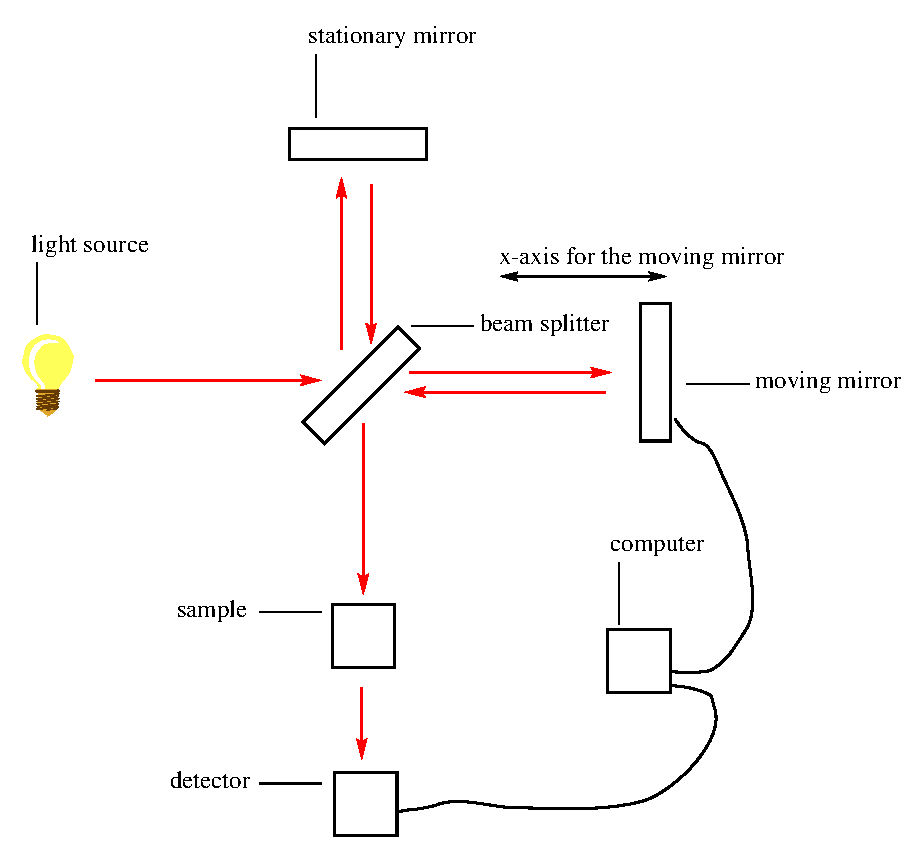
\includegraphics[width=0.7\textwidth] {SkizzeFTIR.eps}
\caption{\label{fig:Skizze1} A simplified version of a Michelson interferometer in a FT-IR spectroscope is illustrated. The polychromatic light of the light source is splitted at the beam splitter and reflected at the stationary and the moving mirror. The polychromatic light radiates through the sample and the not absorbed light will be recorded by the detector. For the interferogram, the detector signal is recorded as a function of the position of the moving mirror. For the calculation of the IR spectrum the computers uses some fourier transformation. All our experimental measurements were taken by a FT-IR spectroscope.} 
\end{figure}

\begin{figure}[H]
\centering
 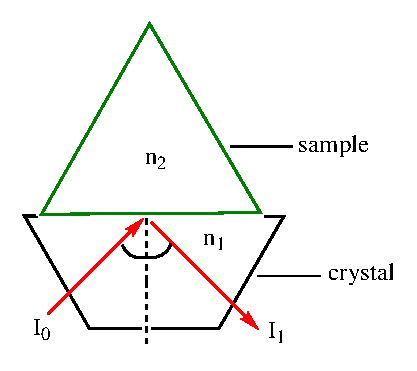
\includegraphics[width=0.25\textwidth] {SkizzeATR.eps}
\caption{\label{fig:Skizze2}A schematic scheme of the ATR module. The entering light beam I$_{0}$ gets totally reflected at the interface of the crystal and the sample on top of it. In the region, where the sample absorbs energy, the evanescent wave will be attenuated. The attenuated beam with intensity I$_{1}$ is than directed to the detector, where the attenuated IR beam is recorded as an interferogram.} 
\end{figure}

All measurements were plotted and the results calculated with Python (Version 3.8) as can be seen in the appendix. 

\newpage
\section*{Results and Discussion}
The measured IR absorption spectrum for ethanol as liquid with its prominent bands is shown in Fig.\ref{fig:TeilA}. The peaks for the characteristic properties of ethanol from the measured IR spectrum compared with a reference IR spectrum are listed below. 

\begin{table}[H]
\centering
\begin{tabular}{c|c|c}
    \thead{measured \\ wavenumber [cm$^{-1}$]} & \thead{reference \\ wavenumber [cm$^{-1}$]} & assignment\cite{assignment} \\
     \hline
    3340 & 3358\cite{IRethanol} & O-H stretch (hydroxyl group) \\
    2974 & 2974\cite{IRethanol} & C-H stretch \\
    1049 & 1050\cite{IRethanol} & C-O stretch (primary alcohol)
\end{tabular}
\end{table}

The measured IR spectrum shows the main significant peaks for the main functional group, the O-H and the C-O stretch of the primary alcohol. The absorption bands match those of the reference spectrum. Therefore a certain measuring accuracy of the measurement instrument can be assumed. 

\begin{figure}[H]
\centering
 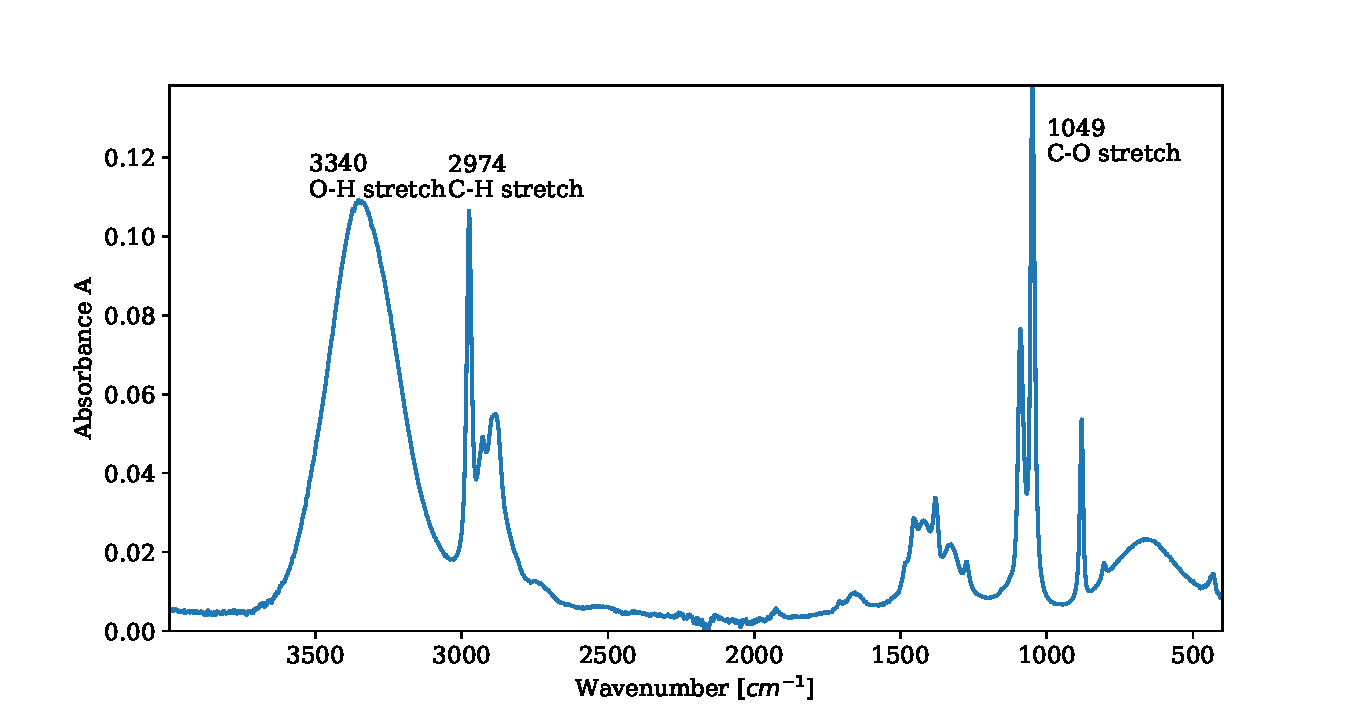
\includegraphics[width=\textwidth] {TeilA.pdf}
\caption{\label{fig:TeilA}The IR spectrum of ethanol as liquid was measured using the ATR module. The characteristic bands for ethanol are labeled in black.} 
\end{figure}

For the analysis of the reproducibility of FT-IR measurements from three samples of liquid ethanol and from three samples of solid benzoic acid an IR spectrum was taken. As can be seen in Fig.\ref{fig:TeilB} the reproductibility of the measurements of the liquid ethanol is better ensured than for the solid benzoic acid. The positions of the individual peaks remain constant for the liquid and the solid samples, but only for the liquid sample the intensity of the absorbance remain nearly consistent as well. The slight differences in the absorbance intensity of the ethanol samples can be neglected, because the cause is probably the fast evaporating of ethanol. The reproductibilty for the measurements with liquid samples can be ensured, but with fast volatile substances, care must be taken that the substances are not exposed to air for too long before the measurement. Before the measurement the solid benzoic acid was mortared leading to different particle sizes, which make the sample less homogeneous. In addition the layer thickness of the solid sample on the measurement instrument differentiated for each of the three measurements. So in conclusion the layer thickness and the concentration of the solid sample was different for the three measurements, which led with inclusion of the Bouger-Lambert-Beer-law (Eq.\ref{eq:A(nu)}) to different absorbance intensities. In order to ensure the reproductibilty of IR spectra with solid samples, the sample preparation and the sample thickness on the measuring plate has to be strictly equal for each measurement.

\begin{figure}[H]
\centering
 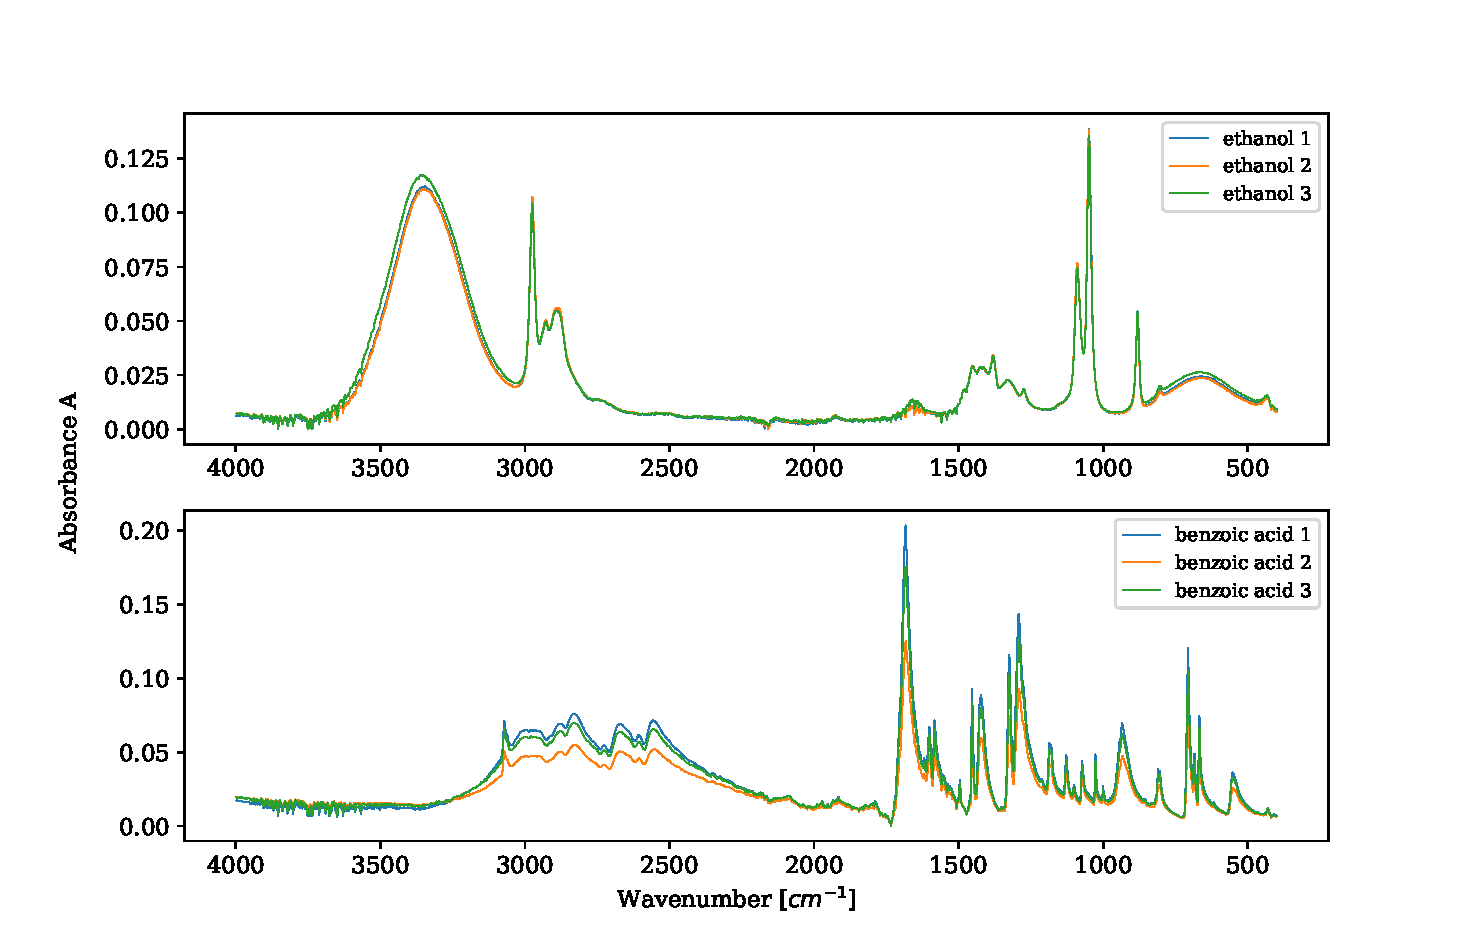
\includegraphics[width=\textwidth] {TeilB.pdf}
\caption{\label{fig:TeilB}The IR spectrum of ethanol as liquid was measured using the ATR module for three times. The sample was replaced after each measurement. The same applies to the solid benzoic acid. For the liquid sample the measurement reproductibility is better ensured than for the solid.} 
\end{figure}

The hydroxyl group has a characteristic peak between 3670 and 2500 cm$^{-1}$\cite{assignment}. For pure DMSO there is no band visible at this range, because the molecule has no hydroxyl group. As can be seen in Fig.\ref{fig:TeilC1} the DMSO contained from the beginning some water as the first measurement at time zero shows a peak at the hydroxyl group region.
The longer DMSO was exposed to ambient air, the more water it absorbed and the stronger the hydroxyl group peak is visible. This confirms the fact that DMSO is a highly hygroscopic substance\cite{DMSO}. At the wavenumber 3442 cm$^{-1}$ the absorbance and the exposition time of all ten measurement were plotted against each other, which is seen in Fig.\ref{fig:TeilC2}. The relation between absorption and time of ambient air exposition was fitted using a fourth degree polynomial function with a confident interval of 0.0003, which confirms the accuracy of the fitted model.

\begin{equation}\label{eq:A(t)}
   {A(t)} = 12(5)\cdot10^{-8} t^{4} - 8(3)\cdot10^{-6}t^{3} + 12(5)\cdot10^{-5}t^{2} + 22(3)\cdot10^{-4} t + 297(5) \cdot10^{-4}
\end{equation}

The fitted function can be seen as an orange graph in Fig.\ref{fig:TeilC2}. After 18 minutes of exposition time the function flattens and the ratio is not linear as in the beginning. DMSO forms hydrogen bonds with water. Over the exposition time all DMSO molecules are saturated with water and no additional hydrogen bonds can be formed. The water absorption of DMSO has a capacity limit, which can be seen with the flattening of the function graph. 

\begin{figure}[H]
\centering
 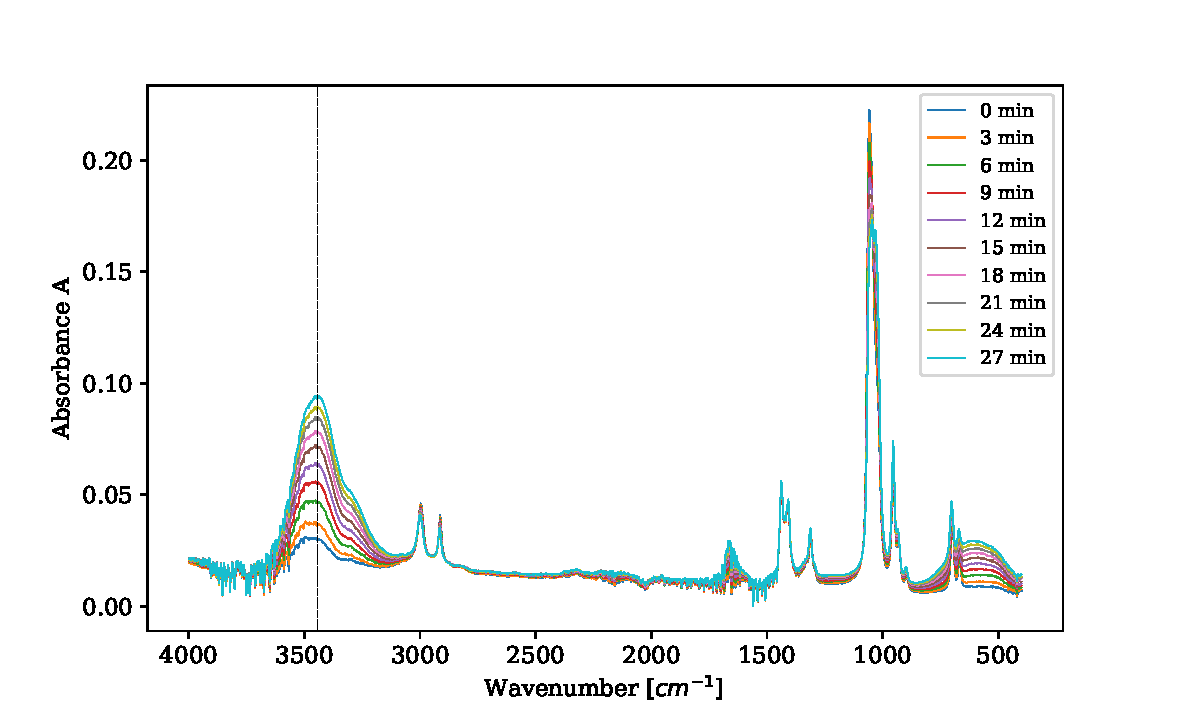
\includegraphics[width=\textwidth] {TeilC1.pdf}
\caption{\label{fig:TeilC1} For 27 minutes after every three minutes an IR spectrum of DMSO, which was not replaced between the measurements, was taken. DMSO is highly hygroscopic and tends to absorb water by exposition to ambient air, which can bee seen with the increasing intensity of the peak for the O-H stretch at wavenumber 3442 cm$^{-1}$ marked by the dashed line.} 
\end{figure}

\begin{figure}[H]
\centering
 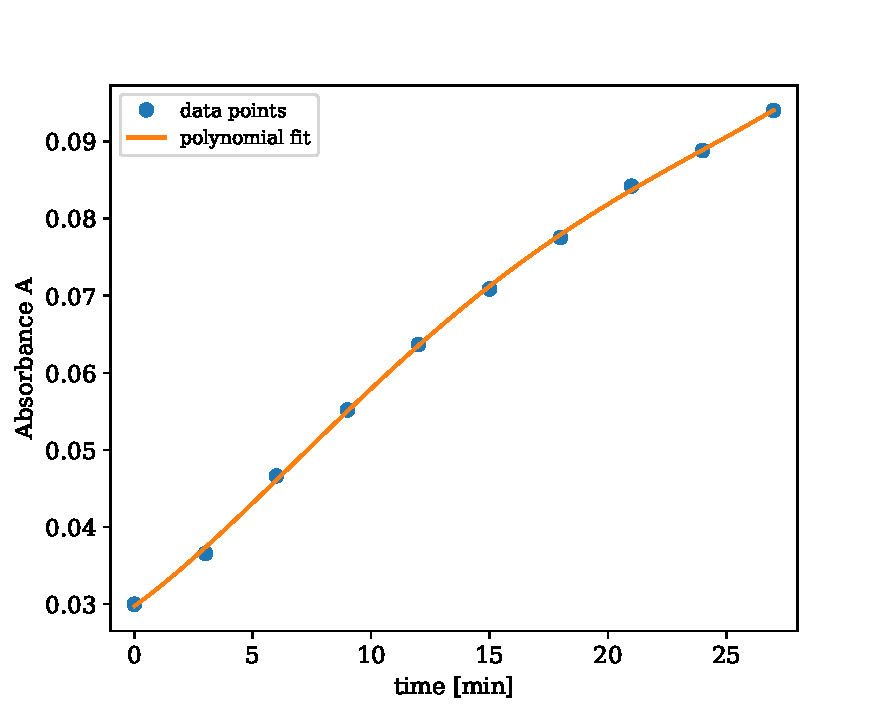
\includegraphics[scale=0.9] {TeilC2.pdf}
\caption{\label{fig:TeilC2} For all ten measurements of DMSO at different times the intensity of the absorbance at wavenumber 3442 cm$^{-1}$ was plotted against the time since DMSO was exposed to ambient air. The longer DMSO was exposed to ambient air, the more water was absorbed, but the relation is not linear. The beginning has a linear ratio, but towards longer exposition to ambient air, the function flattens.}
\end{figure}
\clearpage

The three IR spectra from the polymer samples were compared with spectra from the literature and thereby  their identity was determined. The results can be seen in Tab.\ref{tab:TeilD}. Since all samples could be assigned, IR spectroscopy is a suitable method for the identification of poylmer samples.

\begin{figure}[H]
\centering
 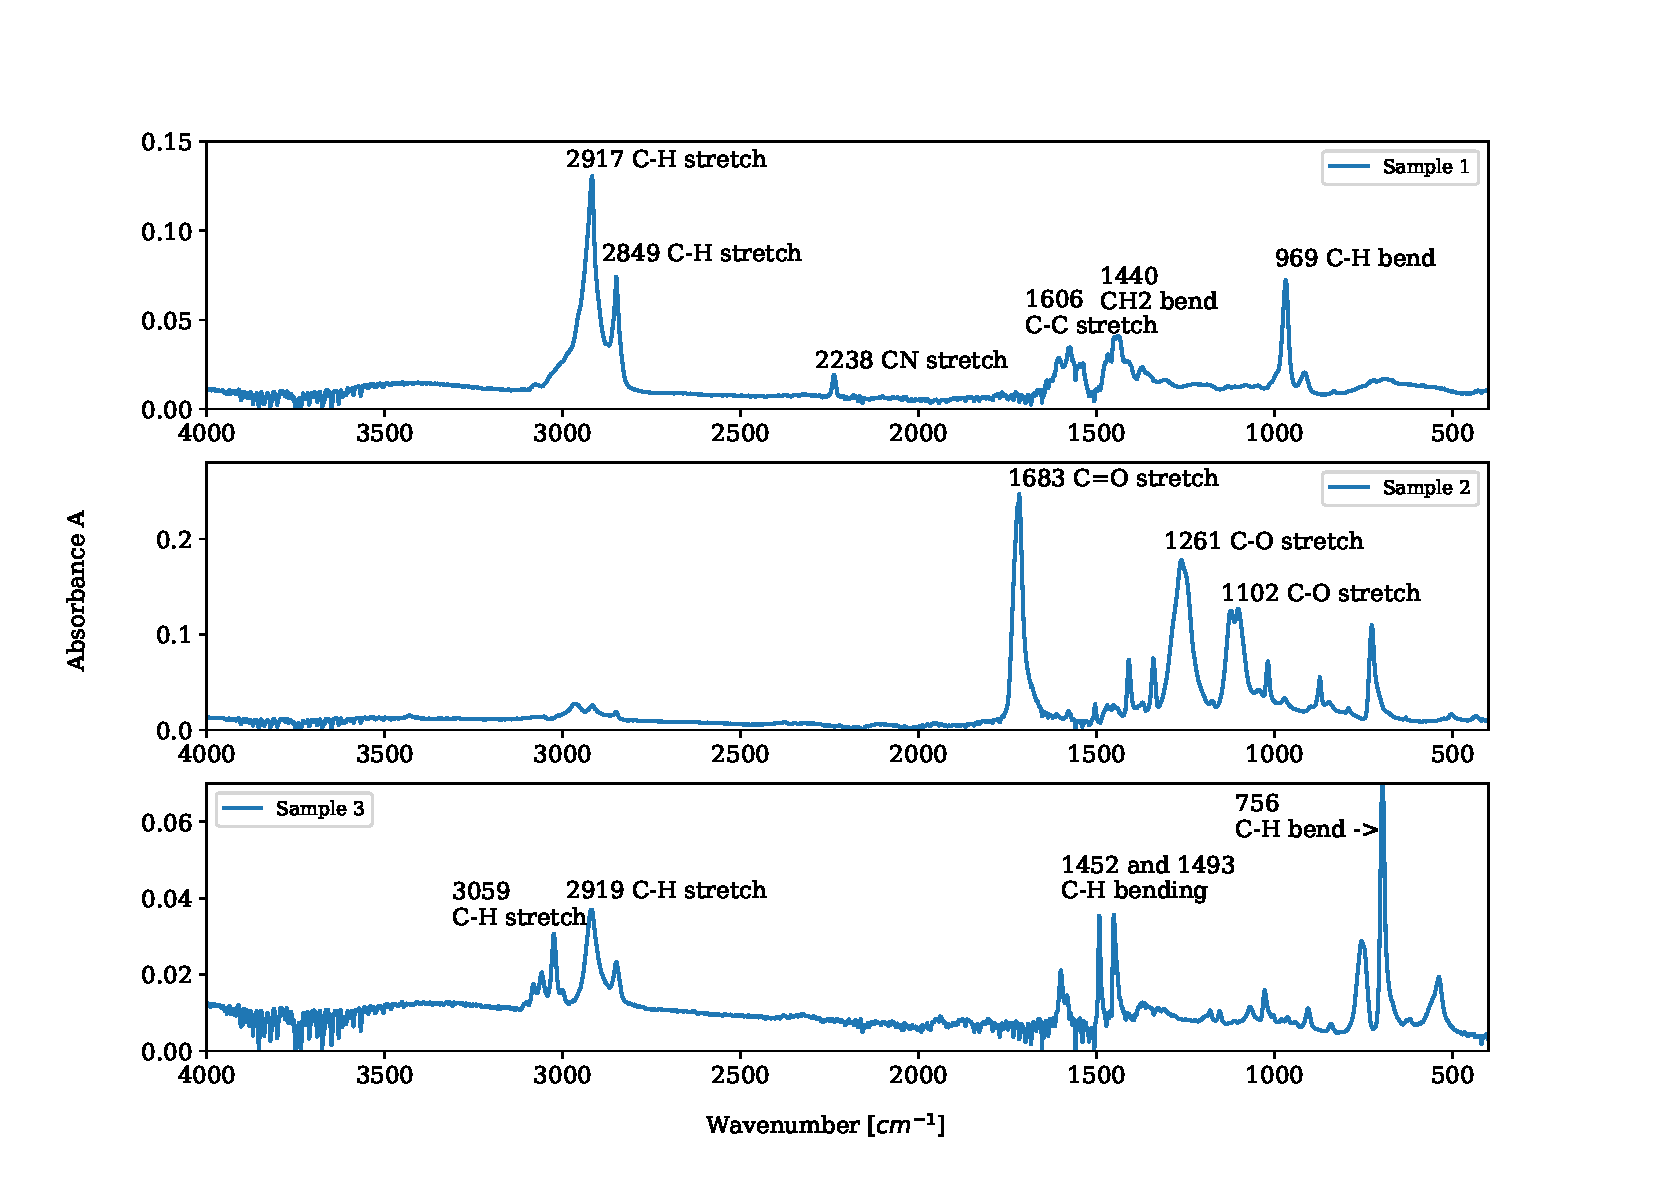
\includegraphics[width=\textwidth] {TeilD.pdf}
\caption{\label{fig:TeilD}From three different polymer sample an IR spectrum was taken using ATR module. The characteristic bands for each sample are labeled in black and further explained in Tab.\ref{tab:TeilD}.} 
\end{figure}

\begin{table}[H]
\centering
\begin{tabular}{c|c|c|c|c}
sample  & identification & \thead{measured \\ wavenumber [cm$^{-1}$]} & \thead{reference \\ wavenumber [cm$^{-1}$]} & assignment\cite{assignment}\\

     \hline
    1 & nitrile & 2917 and 2849 & 2917 and 2849\cite{nitrile}  & C-H stretch \\
    1 & nitrile & 2238 & 2237 \cite{nitrile} & \thead{CN stretch \\ (nitrile)}\\
    1 & nitrile & 1606 & 1605 \cite{nitrile}  & C-C stretch\\
    1 & nitrile & 1440 & 1440 \cite{nitrile} & CH$_{2}$ bend\\
    1 & nitrile & 969 & 967 \cite{nitrile}  & C-H bend\\
    2 & \thead{polyethylene \\ terephthalate} & 1683 & 1730\cite{pet} & C=O stretch \\
    2 & \thead{polyethylene \\ terephthalate} & 1261 & 1285\cite{pet} & \thead{C-O stretch \\ (carboxyl group)}\\
    2 & \thead{polyethylene \\ terephthalate} & 1102 & 1096\cite{pet} &\thead{C-O stretch \\ (ester group)}\\
    3 & polystyrene & 3059 & 3025\cite{poly} & \thead{aromatic \\ C-H stretch}\\
    3 & polystyrene & 2919 & 2921\cite{poly} & C-H stretch\\
    3 & polystyrene & 1452 and 1493 & 1451 and 1493\cite{poly} & \thead{aromatic C-H \\ stretch vibration}\\
    3 & polystyrene & 756 & 749\cite{poly} & \thead{aromatic C-H \\ deformation vibration}
\end{tabular}
\caption{\label{tab:TeilD} The spectral bands from the three polymer samples assigned with their types of oscillation.}
\end{table}

In Fig.\ref{fig:TeilE1} different absorbance spectra from different ethanol/water solutions are presented. It is shown that the absorbance intensity of the O-H peak decreases with increasing ethanol content. The same pattern applies for the fingerprint region between 800 and 600 cm$^{-1}$. The intensity of the O-H peak decreases with increasing ethanol content, because ethanol has only one O-H bond and therefore less hydrogen bonds and O-H bonds can cause oscillation in the region between 3550 and 2500 cm$^{-1}$\cite{assignment}. Unlike water, ethanol has C-H bonds in its molecule structure, which causes increasing peak intensities at 2975 and 2890 with rising ethanol content. The wavenumbers 3384, 2975 and 692 cm$^{-1}$ were selected to generate a function to calculate the ethanol content dependant on the absorbance intensity at these specific wavenumbers. Using the calibration points with the known ethanol contents a linear model was fitted using linear regression, which can be seen in Fig.\ref{fig:TeilE2}. The results of the ethanol content determination from three alcohol samples are shown in Tab.\ref{tab:TeilE}.

\begin{figure}[H]
\centering
 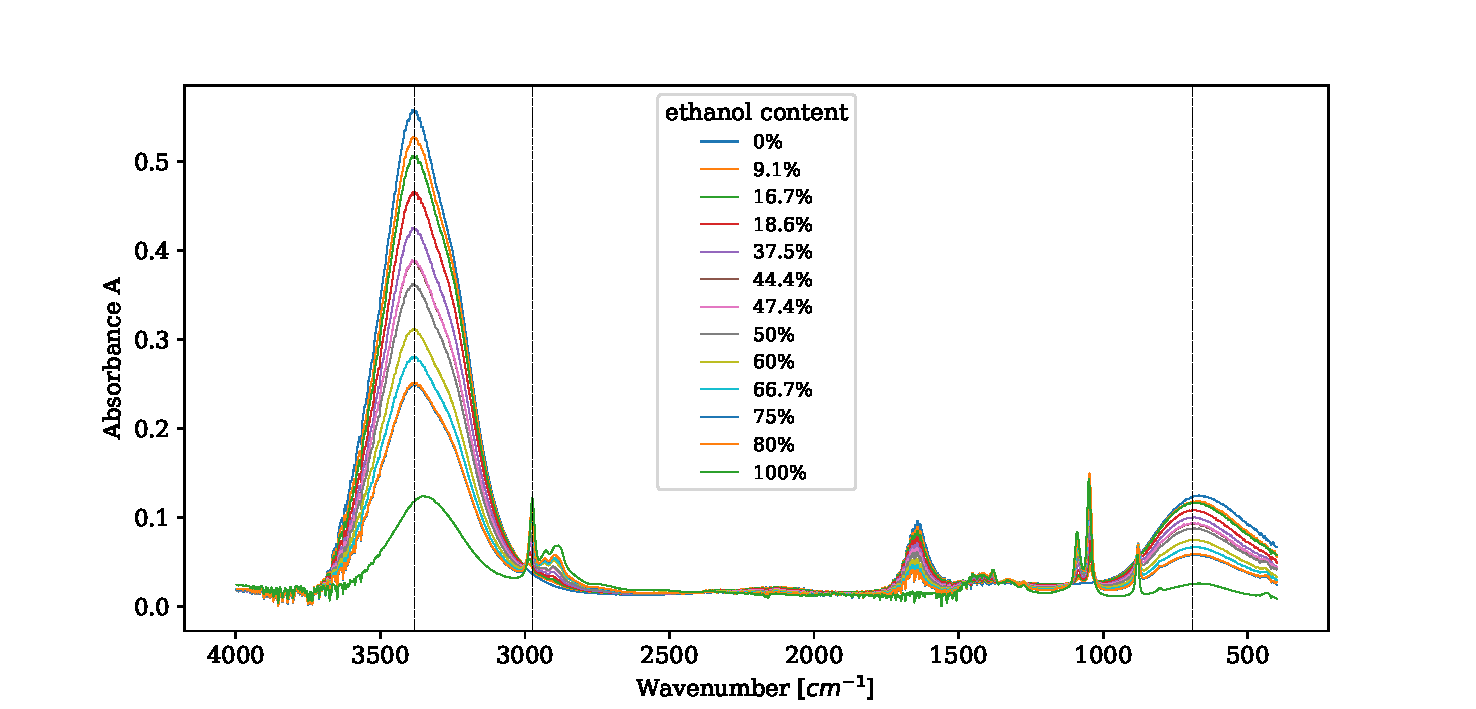
\includegraphics[width=1\textwidth] {TeilE1.pdf}
\caption{\label{fig:TeilE1}From known solutions with different ethanol and water contents IR spectra were measured. The higher the ethanol content of the solution the less the intensity of the O-H peak at wavenumber 3384 cm$^{-1}$ is visible. The same pattern applies in the fingerprint region at wavenumber 692 cm$^{-1}$. In return the C-H peak at wavenumber 2975 cm$^{-1}$ increases with higher ethanol content. The changes in the band intensities at these three wavenumbers, which are marked with dashed lines, were used to determine the ethanol content of three different alcohol samples.}
\end{figure}

\begin{table}[H]
\centering
\begin{tabular}{c|c|c|c}
    linear model & alcohol sample  & \thead{calculated ethanol \\ content [vol\%]} & \thead{reference ethanol \\ content [vol\%]}\\
     \hline
    at O-H peak region & white wine & 16.2 $\pm$ 1.8 & 13.5\\
    at O-H peak region & anise & 39.3 $\pm$ 1.8 & 35\\
    at O-H peak region & rum & 36.4 $\pm$ 1.8 & 40\\
     \hline
    at C-H peak region & white wine & 18.1 $\pm$ 2.4 & 13.5\\
    at C-H peak region & anise & 46.0 $\pm$ 2.4 & 35\\
    at C-H peak region & rum & 36.9 $\pm$ 2.4 & 40\\
     \hline
    at fingerprint region & white wine & 14 $\pm$ 3 & 13.5\\
    at fingerprint region & anise & 37 $\pm$ 3 & 35\\
    at fingerprint region & rum & 34 $\pm$ 3 & 40\\
\end{tabular}
\caption{\label{tab:TeilE} In this table the results from the ethanol content determination of three alcohol samples is shown. The used linear model can be seen in Fig.\ref{fig:TeilE2}.The reference ethanol contents were provided from the assistent Luis F\'abregas Ib\'a\~nez.}
\end{table}

The calculated means and standard deviations for the three alcohol samples are for the white wine 16 $\pm$ 1$\%$, for the rum 36 $\pm$ 1$\%$ and for the anise 40.8 $\pm$ 2.2$\%$. 
The calculations at the fingerprint region are the most truthful, because except for the rum the other two results fall within the confidence interval. It seems like the samples anise and rum interchanged, because rum should have the higher ethanol content than anise. Perhaps before the anise measurement the ethanol for cleaning the measurement instrument was not completely evaporated and therefore increased the ethanol content of the anise sample. The low percentage of the rum sample could be explained as the measurement was not taken immediately after the sample was placed on the measurement instrument and some ethanol evaporated before the measurement. For the inaccurate results from all three samples has to be considered that the alcohol samples not only contain water and ethanol. Therefore the other ingredients can falsify the calculations, because the calibration function is based on water/ethanol solutions. In addition certain inaccuracies could be caused through the sample preparation of the water/ethanol samples and the measuring of the IR spectra from these samples. Ethanol is volatile and therefore by the sample preparation due to not fast enough closing of the sample containers some ethanol could have evaporated. After every ethanol/water sample measurement the measuring instrument was cleaned with ethanol. If not all of the ethanol evaporated it could have mixed up with the ethanol/water samples and increased their ethanol content. 

\begin{figure}[H]
\centering
 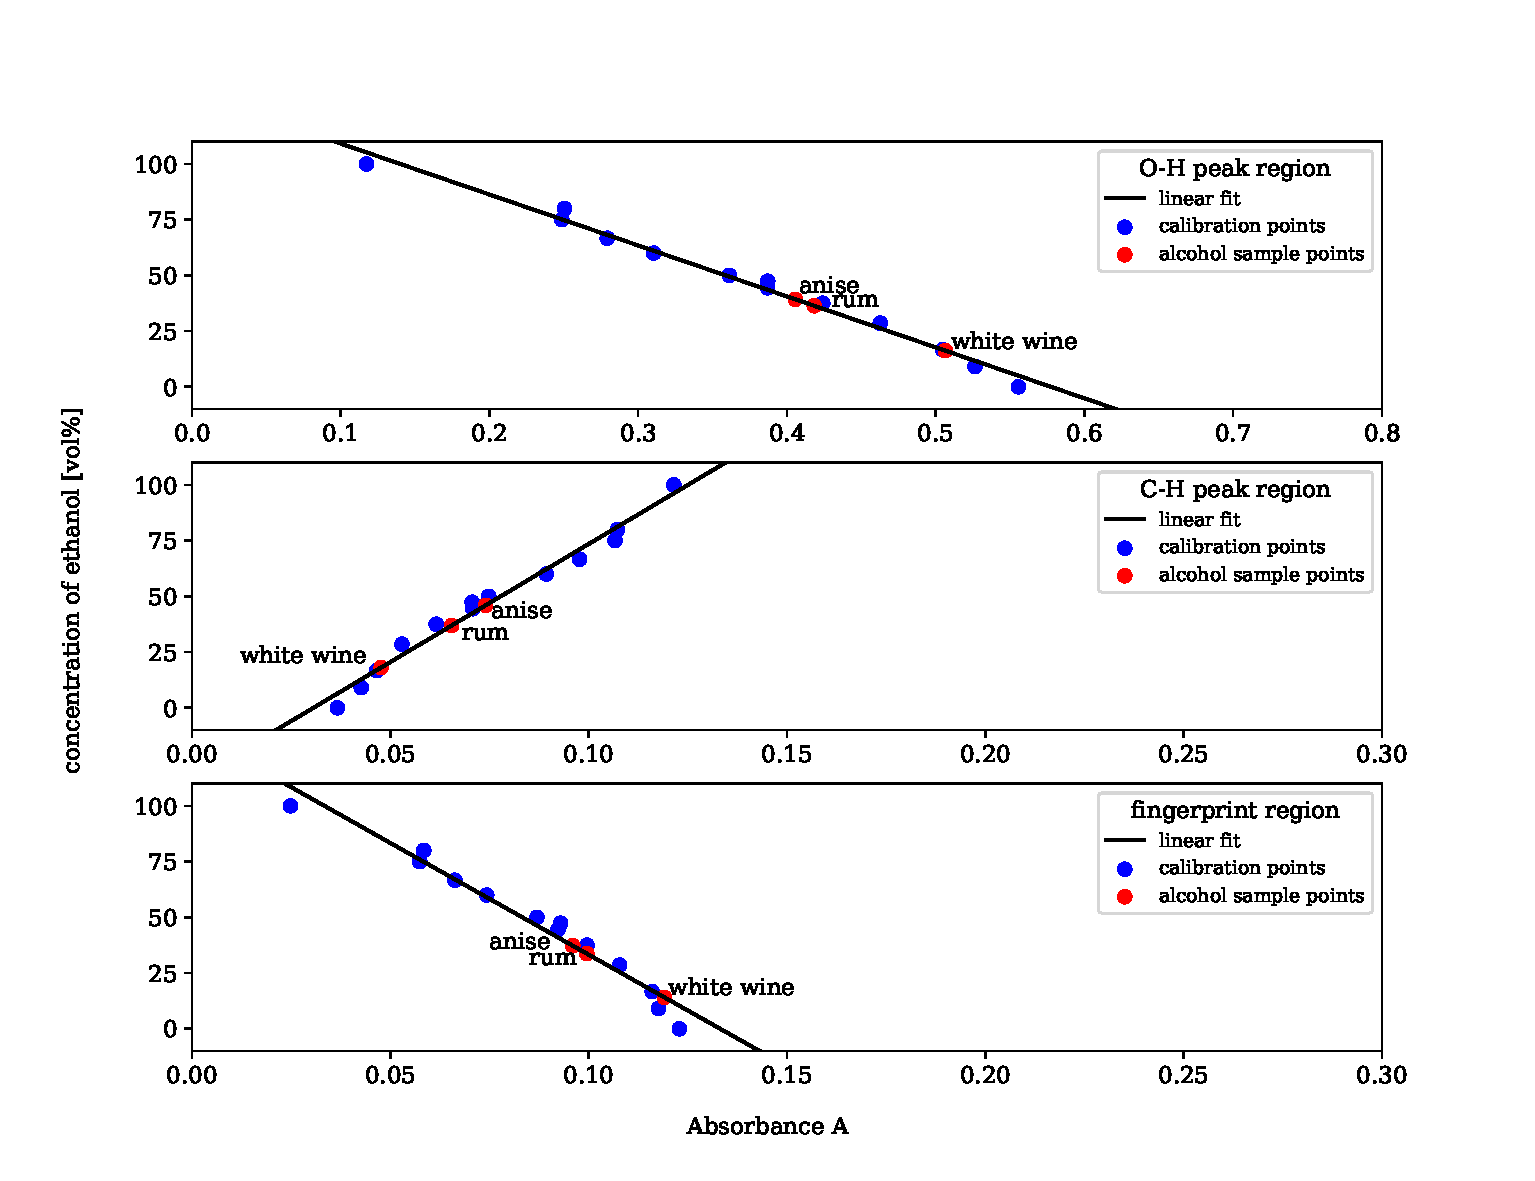
\includegraphics[width=\textwidth] {TeilE2.pdf}
\caption{\label{fig:TeilE2}From the IR spectra from the ethanol and water solutions, which can be seen in Fig.\ref{fig:TeilE1} at three specific wavenumbers, namely 3384, 29475 and 692 cm$^{-1}$, the absorbance was plotted against the ethanol content. The ratios at all three wavenumbers were linear and therefore using linear regression a calibration function was determined. Using the calibration function the ethanol content of three samples was calculated.}
\end{figure}
\clearpage

The absorption spectra of \ce{H2O} and \ce{D2O} are shown in Fig.\ref{fig:TeilF}. The absorption spectra show the same absorption pattern, but their peaks positions are shifted. The shifts are caused upon isotopic substitution, since deuterium oxide has the higher reduced mass than water. The O-D peak is shifted to the right compared to the O-H peak. The O-H peak is at wavenumber 3389 cm$^{-1}$ and the O-D peak at wavenumber 2496 cm$^{-1}$. Therefore the O-H peak is shifted by a value of 0.737. By transforming Eq.\ref{eq:TeilF1} under the assumption that the spring constant for the O-H and O-D bond is equal the shift of the vibration wavenumber can be calculated as

\begin{equation}\label{eq:F2}
   {\frac{\tilde{\nu}_{O-D}}{\tilde{\nu}_{O-H}}} = \sqrt{\frac{16 + 2}{16 \cdot 2} \cdot \frac{16 \cdot 1}{16 + 1}} = 0.728.
\end{equation}

Comparing the calculated shift number of 0.728 with the experimentally determined shift number of 0.737 it can be assumed that the measured absorption peaks of the O-H and the O-D band are accurate. 

\begin{figure}[H]
\centering
 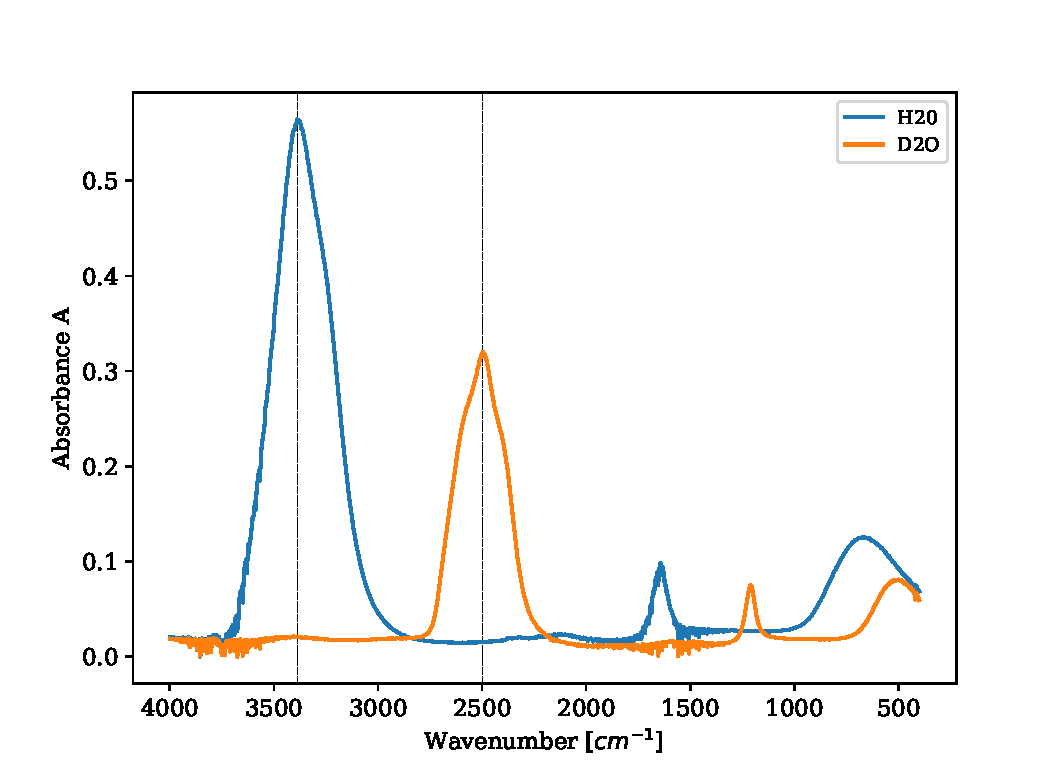
\includegraphics[width=\textwidth] {TeilF.pdf}
\caption{\label{fig:TeilF}From distilled water and deuterium oxide IR spectra using ATR module were taken. The peak for the O-H stretch is at 3389 cm$^{-1}$ and the peak for the O-D stretch at 2496 cm$^{-1}$, which is marked by the dashed lines. The peak for the O-D stretch is at a lower wavenumber, because deuterium oxide has the bigger reduced mass than distilled water.}
\end{figure}
\clearpage

 An excerpt of the gaseous absorption spectrum of \ce{HBr}, which can be seen in Fig.\ref{fig:TeilG}, shows the fundamental band with its transition wavenumbers of the P- and R-branches. The transition wavenumbers of the P- and R-branches of the fundamental band are linear dependant on the coefficients q1, q2 and q3.
 
\begin{equation}\label{eq:GR}
   \tilde{\nu} = B_{e}q1 - \alpha q2 - D_{e}q3 + \tilde{\nu}_{0}
\end{equation}

The coefficients q1, q2 and q3 can be calculated from the vibration and rotation levels of the transition wavenumbers as

\begin{equation}\label{eq:Gq}
    \begin{split}
   q1 = J'(J' + 1) - J''(J'' + 1) \\\
   q2 = (1 (\nu = 1) + \frac{1}{2})J'(J' + 1) - \frac{1}{2}J''(J'' + 1) \\\
   q3 = (J'(J' + 1))^2 - (J''(J'' + 1))^2,
   \end{split}
\end{equation}

which comes from the Eq.\ref{eq:TeilG1} and the results can be seen in Tab.\ref{tab:TeilG}. Since only the fundamental band is analyzed the first two arguments in Eq.\ref{eq:TeilG1} results in $\tilde{\nu}_{0}$, which is the intercept of Eq.\ref{eq:GR}. A multiple linear regression was used to determine the rotational constant B$_{e}$, which resulted in 8.463 $\pm$ 0.016 cm$^{-1}$. Using Eq.\ref{eq:TeilG2} the bond length of \ce{HBr} could be determined as 142 \p m. In comparison with the value in literature of 141 \p m\cite{HBr} the calculations were accurate.

\begin{table}[H]
\centering
\begin{tabular}{c|c|c|c|c}
    transition state & wavenumber [cm$^{-1}$] & q1 & q2 & q3\\
     \hline
    R(0) & 2575 & 2 & 3 & 4\\
    R(1) & 2591 & 4 & 8 & 32\\
    R(2) & 2606 & 6 & 15 & 108\\
     \hline
    P(1) & 2542 & -2 & -1 & -4\\
    P(2) & 2525 & -4 & 0 & -32\\
    P(3) & 2507 & -6 & 3 & -108\\
\end{tabular}
\caption{\label{tab:TeilG} The transition wavenumber of three R- and P-branches and the coefficients calculated from the vibration and rotation quantum numbers of the involved states are shown. The coefficients and the transition wavenumbers were used for the determination of the the rotation constant $B_{e}$ of the molecule \ce{HBr}. }
\end{table}


\begin{figure}[H]
\centering
 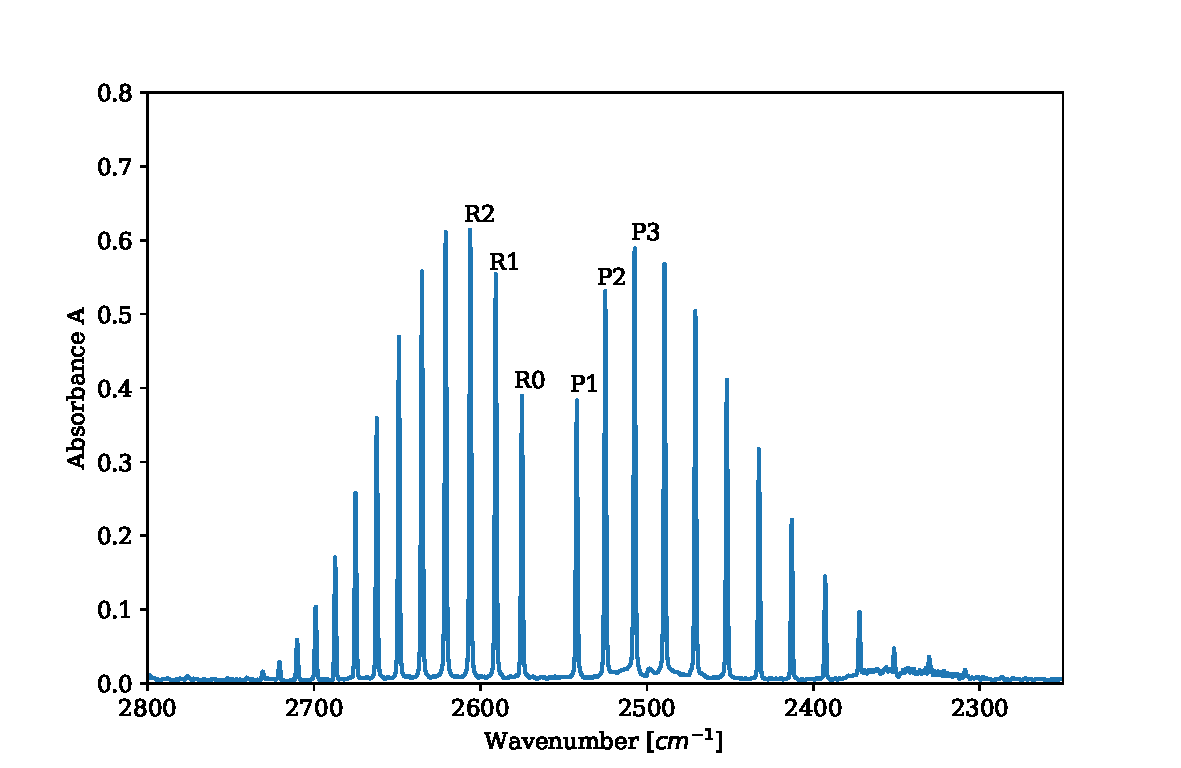
\includegraphics[width=\textwidth] {TeilG.pdf}
\caption{\label{fig:TeilG}The for the calculation of the bond length relevant cutout of the gaseous \ce{HBr} absorption spectrum, which was measured with the transmission method, is shown. The spectrum was provided from the assistant Luis F\'abregas Ib\'a\~nez. The for the calculation used R- and P-branch transition states are labeled in black.}
\end{figure}

\pagebreak

\setcounter{biburllcpenalty}{7000}
\setcounter{biburlucpenalty}{8000}
%\Urlmuskip=0mu plus 10mu
\printbibliography
%\balance
 
\newpage 
  
\section*{Appendix}
A1 - Python Scripts\\
A2 - Lab journal, dated March 30 2021.\\
A3 - Task sheet \\
A4 - Regression summaries


\subsection*{A1 - Python Scripts}

\subsubsection*{Python Code for part A}
\begin{lstlisting}[language=Python]
import numpy as np
from scipy import stats as stats
import matplotlib.pyplot as plt
from scipy.optimize import leastsq
from scipy.signal import find_peaks

filename = 'Ethanol.dpt'

font = {'family' : 'serif',
        'weight' : 'normal',
        'size'   : 11}
plt.rc('font', **font)
Smallsize = 11
cm = 1/2.54
 
data = np.loadtxt(filename, delimiter=',', skiprows=1, dtype=float)
y = data[:,1]
x = data[:,0]
fig, ax = plt.subplots(figsize=(23*cm, 12*cm),dpi=600)  
ax.text(3045,0.10985,"2974 \nC-H stretch")
ax.text(3521,0.11000,"3340 \nO-H stretch")
ax.text(1000,0.11900,"1049 \nC-O stretch")
plt.rc('font', size=Smallsize)          # controls default text sizes
plt.rc('axes', labelsize=Smallsize)    # fontsize of the x and y labels
plt.rc('legend', fontsize=9)  
plt.ylabel(r'Absorbance A')
plt.xlabel('Wavenumber [$cm^{-1}$]')
peaks, properties  = find_peaks(y,height=0.1)
Peakpunkte = data[peaks]
plt.plot(x,y)
plt.axis([max(x),min(x),min(y),max(y)])
plt.savefig('TeilA.pdf')
plt.show()
\end{lstlisting}

\subsubsection*{Python Code for part B}
\begin{lstlisting}[language=Python]
import numpy as np
from scipy import stats as stats
import matplotlib.pyplot as plt
from scipy.optimize import leastsq
from scipy.signal import find_peaks

font = {'family' : 'serif',
        'weight' : 'normal',
        'size'   : 11}
plt.rc('font', **font)
Smallsize = 11
plt.rc('font', size=Smallsize)          # controls default text sizes
plt.rc('axes', labelsize=Smallsize)    # fontsize of the x and y labels
plt.rc('legend', fontsize=9)  
cm = 1/2.54

fig, ax = plt.subplots(2,1,figsize=(25*cm, 16*cm),dpi=600)   
fig.text(0.5, 0.04, 'Wavenumber [$cm^{-1}$]', ha='center')
fig.text(0.04, 0.5, r'Absorbance A', va='center', rotation='vertical')
filenamesEthanol = ['B1_Ethanol.dpt','B2_Ethanol.dpt','B3_Ethanol.dpt']
filenamesBenz = ['B1_Benzoesaeure.dpt','B2_Benzoesaeure.dpt','B3_Benzoesaeure.dpt']
dataframesEthanol = []
labelse = ['ethanol 1','ethanol 2','ethanol 3']
labelsb = ['benzoic acid 1','benzoic acid 2','benzoic acid 3']
dataframesBenz= []
n = [0,1,2]
for i,f,k,l,m in zip(n,filenamesEthanol,filenamesBenz,labelsb,labelse):
    dataframesEthanol.append(np.loadtxt(f, delimiter=',', skiprows=1, dtype=float))
    dataframesBenz.append(np.loadtxt(k, delimiter=',', skiprows=1, dtype=float))
    y = dataframesEthanol[i][:,1]
    x = dataframesEthanol[i][:,0]
    ax[0].plot(x,y,label = m,linewidth = 0.5)
    ax[0].legend()
    y = dataframesBenz[i][:,1]
    x = dataframesBenz[i][:,0]
    ax[1].plot(x,y,label = l,linewidth = 0.5)
    ax[1].legend()

ax[0].invert_xaxis()
ax[1].invert_xaxis()
plt.show
plt.savefig('TeilB.pdf')
\end{lstlisting}
\subsubsection*{Python Code for part C}
\begin{lstlisting}[language=Python]

import numpy as np
import statsmodels.formula.api as smf
import pandas as pd
from scipy import stats as stats
import matplotlib.pyplot as plt
from scipy.optimize import leastsq
from scipy.signal import find_peaks

font = {'family' : 'serif',
        'weight' : 'normal',
        'size'   : 1}
plt.rc('font', **font)
Smallsize = 11
plt.rc('font', size=Smallsize)          # controls default text sizes
plt.rc('axes', labelsize=Smallsize)    # fontsize of the x and y labels
plt.rc('legend', fontsize=9)  
cm = 1/2.54
fig, ax = plt.subplots(figsize=(20*cm, 12*cm),dpi=600)   
filenames = ['C1_DMSO.dpt','C2_DMSO.dpt','C3_DMSO.dpt','C4_DMSO.dpt','C5_DMSO.dpt','C6_DMSO.dpt','C7_DMSO.dpt','C8_DMSO.dpt','C9_DMSO.dpt','C10_DMSO.dpt']
labels = ['0 min',"3 min","6 min","9 min", "12 min", "15 min", "18 min", "21 min", "24 min", "27 min"]
dataframes = []
n = [0,1,2,3,4,5,6,7,8,9]
for i,f,l in zip(n,filenames,labels):
    dataframes.append(np.loadtxt(f, delimiter=',', skiprows=1, dtype=float))
    y = dataframes[i][:,1]
    x = dataframes[i][:,0]
    x1 = dataframes[i][545,0]
    ax.plot(x,y,label=l,linewidth = 0.5)
    ax.axvline(x1, color='k', linestyle='--',linewidth = 0.4)
    ax.legend()
    ax.set_ylabel(r'Absorbance A')
    ax.set_xlabel('Wavenumber [$cm^{-1}$]')
  
ax.invert_xaxis()
plt.savefig('TeilC1.pdf')


#Unterschied = 10 verschiedene Absorbanzen bei Wellenlänge 3441.65
Unterschied = np.zeros((10,2))
for i in range(0,10):
    Unterschied[i] = dataframes[i][545]
fig, ax = plt.subplots(figsize=(15*cm, 12*cm),dpi=600)  
fity = Unterschied[:,1]
fitx = np.array([0,3,6,9,12,15,18,21,24,27])
# Koeffizienten berechnen
coeffs,cov = np.polyfit(fitx, fity, 4, cov = True)
# macht Polynom für Plot 
poly = np.poly1d(coeffs)
new_x = np.linspace(fitx[0], fitx[-1])
new_y = poly(new_x) 
# gemessenen X-Werte in Polynomfunktion eingesetzt
y_val = poly(fitx)
plt.xlabel(r'time [min]')
plt.ylabel(r'Absorbance A')
plt.plot(fitx, fity, "o", label ='data points')
plt.plot(new_x, new_y, label = 'polynomial fit')
plt.xlim([fitx[0]-1, fitx[-1] + 1 ]) 
plt.rc('font', size=Smallsize)          # controls default text sizes
plt.rc('axes', labelsize=Smallsize)    # fontsize of the x and y labels
plt.rc('legend', fontsize=9)   
plt.legend()
plt.savefig('TeilC2.pdf')
plt.show

"""
Vertrauensintervall Berechnung
"""
# Standardfehler Mittelwert
n = np.std(fity-y_val)/np.sqrt(10)
#t-taktil 
ts = stats.t(df=9).ppf(0.975)
Verintervall = n*ts 

"""""
Standardfehler für die einzelnen Coeffs
"""
Standardfehlercoeffs = np.sqrt(np.diag(cov))
print('Standardfehler t^4, t^3, t^2, t und Steigung:\n',Standardfehlercoeffs)
\end{lstlisting}
\subsubsection*{Python Code part D}
\begin{lstlisting}[language=Python]
import numpy as np

from scipy import stats as stats
import matplotlib.pyplot as plt
from scipy.optimize import leastsq
from scipy.signal import find_peaks

font = {'family' : 'serif',
        'weight' : 'normal',
        'size'   : 1}
plt.rc('font', **font)
Smallsize = 11
plt.rc('font', size=Smallsize)          # controls default text sizes
plt.rc('axes', labelsize=Smallsize)    # fontsize of the x and y labels
plt.rc('legend', fontsize=9)  
cm = 1/2.54

fig, ax = plt.subplots(3,1,figsize=(28*cm, 20*cm),dpi=600)  
fig.text(0.5, 0.04, 'Wavenumber [$cm^{-1}$]', ha='center')
fig.text(0.04, 0.5, r'Absorbance A', va='center', rotation='vertical') 

Handschuh = ['D1_Handschuh.dpt']
PET = ['D2_PET.dpt']
CD = ['D3_CD.dpt']
dataframesHandschuh = []
dataframesPET = []
dataframesCD = []
n = [0]
for i,f,k,m in zip(n,Handschuh,PET,CD):
    dataframesHandschuh.append(np.loadtxt(f, delimiter=',', skiprows=1, dtype=float))
    dataframesPET.append(np.loadtxt(k, delimiter=',', skiprows=1, dtype=float))
    dataframesCD.append(np.loadtxt(m, delimiter=',', skiprows=1, dtype=float))
    y = dataframesHandschuh[i][:,1]
    x = dataframesHandschuh[i][:,0]
    peaks, properties  = find_peaks(y,height=None)
    Peakpunkte = dataframesHandschuh[i][peaks]
    ax[0].axis([400, 4000, 0, 0.15])
    ax[0].plot(x,y,label = 'Sample 1')
    ax[0].text(2990,0.13600,"2917 C-H stretch")
    ax[0].text(2890,0.08285,"2849 C-H stretch")
    ax[0].text(2290,0.02300,"2238 CN stretch")
    ax[0].text(1700,0.04280,"1606 \nC-C stretch")
    ax[0].text(1490,0.05600,"1440 \nCH2 bend")
    ax[0].text(1000,0.08000,"969 C-H bend")
    ax[0].legend()
    y = dataframesPET[i][:,1]
    x = dataframesPET[i][:,0]
    #peaks, properties  = find_peaks(y,height=0.02)
    #Peakpunkte = dataframesPET[i][peaks]
    ax[1].axis([400, 4000, 0, 0.28])
    ax[1].plot(x,y,label = 'Sample 2')
    ax[1].text(1750,0.255,"1683 C=O stretch")
    ax[1].text(1310,0.19,"1261 C-O stretch")
    ax[1].text(1150,0.135,"1102 C-O stretch")
    ax[1].legend()
    y = dataframesCD[i][:,1]
    x = dataframesCD[i][:,0]
    #peaks, properties  = find_peaks(y,height=0.02)
    #Peakpunkte = dataframesPET[i][peaks]
    ax[2].axis([400, 4000, 0, 0.07])
    ax[2].plot(x,y,label = 'Sample 3')
    ax[2].text(3310,0.033,"3059 \nC-H stretch")
    ax[2].text(2990,0.04,"2919 C-H stretch")
    ax[2].text(1600,0.04,"1452 and 1493 \nC-H bending")
    ax[2].text(1110,0.056,"756 \nC-H bend ->")
    ax[2].legend()

ax[0].invert_xaxis()
ax[1].invert_xaxis()
ax[2].invert_xaxis()
plt.savefig('TeilD.pdf')
plt.show
\end{lstlisting}
\subsubsection*{Python Code part E}
\begin{lstlisting}[language=Python]
import numpy as np
from scipy import stats as stats
import matplotlib.pyplot as plt
from scipy.optimize import leastsq
from scipy.signal import find_peaks

"""
Grösseneinstellungen / Schrifteinstellungen
"""
font = {'family' : 'serif',
        'weight' : 'normal',
        'size'   : 11}
plt.rc('font', **font)
Smallsize = 11
cm = 1/2.54
"""
Daten für die Kalibration mit den bekannten Ethanolgehältern
"""
fig, ax = plt.subplots(figsize=(25*cm, 12*cm),dpi=600) 
filenames = ['E1.dpt','E2.dpt','E3.dpt','E4.dpt','E5.dpt','E6.dpt','E7.dpt','E8.dpt','E9.dpt','E10.dpt','E11.dpt','E12.dpt','E13.dpt']
labels = ['0%','9.1%','16.7%','18.6%','37.5%','44.4%','47.4%','50%','60%','66.7%','75%','80%','100%']
dataframes = []
n = [0,1,2,3,4,5,6,7,8,9,10,11,12]
for l,i,f in zip(labels,n,filenames):
    dataframes.append(np.loadtxt(f, delimiter=',', skiprows=1, dtype=float))
    y = dataframes[i][:,1]
    x = dataframes[i][:,0]
    plt.rc('font', size=Smallsize)          # controls default text sizes
    plt.rc('axes', labelsize=Smallsize)    # fontsize of the x and y labels
    plt.rc('legend', fontsize=9)  
    ax.plot(x,y, label = l, linewidth = 0.5)
    x1 = dataframes[i][602,0]
    x2 = dataframes[i][1003,0]
    x3 = dataframes[i][3241,0]
    ax.axvline(x1, color='k', linestyle='--',linewidth = 0.4)
    ax.axvline(x2, color='k', linestyle='--',linewidth = 0.4)
    ax.axvline(x3, color='k', linestyle='--',linewidth = 0.4)
    plt.legend(title="ethanol content")
    ax.set_ylabel(r'Absorbance A')
    ax.set_xlabel('Wavenumber [$cm^{-1}$]')   
ax.invert_xaxis()
plt.savefig('TeilE1.pdf')

"""
Daten der zu bestimmenden Substanzen
"""
fig, ax = plt.subplots(figsize=(12, 4))   
filenames2 = ['E_Rum.dpt','E_Weisswein.dpt','E_Anise.dpt']
dataframes2 = []
m = [0,1,2]
for i,f in zip(m,filenames2):
    dataframes2.append(np.loadtxt(f, delimiter=',', skiprows=1, dtype=float))
    y = dataframes2[i][:,1]
    x = dataframes2[i][:,0]
    ax.plot(x,y)
    ax.set_ylabel(r'Absorbance')
    ax.set_xlabel('Wavenumber [$cm^{-1}$]')   
ax.invert_xaxis()
plt.show
plt.figure()
"""
Modelfunktionberechnung:
    -bei Wellenlänge 3383.52, bei Index 602 für OH stretch 
    -bei Wellenlänge 2974.6, bei Index 1003 für CH stretch
    -bei Wellenlänge 692.409, bei Index 3241 in Fingerprint Region
"""
Unterschied = np.zeros((13,2))
Unterschied1 = np.zeros((13,2))
Unterschied2 = np.zeros((13,2))
for i in range(0,13):
    Unterschied[i] = dataframes[i][602]
    Unterschied1[i] = dataframes[i][1003]
    Unterschied2[i] = dataframes[i][3241]
Samples = np.zeros((3,2))   
Samples1 =np.zeros((3,2)) 
Samples2 =np.zeros((3,2))
for i in range(0,3):
    Samples[i] = dataframes2[i][602]
    Samples1[i] = dataframes2[i][1003]
    Samples2[i] = dataframes2[i][3241]
    
fig, ax = plt.subplots(3,1,figsize=(26*cm, 20*cm),dpi=600)  
plt.rc('font', size=Smallsize)          # controls default text sizes
plt.rc('axes', labelsize=Smallsize)    # fontsize of the x and y labels
plt.rc('legend', fontsize=9)  
fig.text(0.5, 0.04, r'Absorbance A', ha='center')
fig.text(0.04, 0.5, 'concentration of ethanol [vol%]', va='center', rotation='vertical')
# X Achse die verschiedenen Absorbanzen, Y Achse gibt den Ethanolgehalt
fitx = Unterschied[:,1]
fitx1 = Unterschied1[:,1]
fitx2 = Unterschied2[:,1]
fitxSample = Samples[:,1]
fitxSample1 = Samples1[:,1]
fitxSample2 = Samples2[:,1]
fity = np.array([0,100/110*10,100/120*20,100/140*40,100/160*60,100/180*80,100/190*90,50,100/250*150,100/300*200,100/400*300,100/500*400,100])
# Line fitting 
model,cov = np.polyfit(fitx,fity,1,cov = True)
model1,covv = np.polyfit(fitx1,fity,1,cov = True)
model2,covvv = np.polyfit(fitx2,fity,1, cov = True)
predict = np.poly1d(model)
predict1 = np.poly1d(model1)
predict2 = np.poly1d(model2)
x_lin_reg = np.linspace(0, 1,1000)
y_lin_reg = predict(x_lin_reg)
y_lin_reg1 = predict1(x_lin_reg)
y_lin_reg2 = predict2(x_lin_reg)
y_val = predict(fitx)
y_val1 = predict1(fitx1)
y_val2 = predict2(fitx2)
y_Samples = predict(fitxSample)
y_Samples1 = predict1(fitxSample1)
y_Samples2 = predict2(fitxSample2)
ax[0].axis([0, 0.8, -10, 110])
ax[0].scatter(fitx, fity, c = 'b', label = 'calibration points')
ax[0].scatter(fitxSample, y_Samples, c = 'r', label = 'alcohol sample points')
ax[0].plot(x_lin_reg, y_lin_reg, c = 'k', label = 'linear fit')
ax[0].annotate("white wine", (0.51, 17))
ax[0].annotate("rum", (0.43,36 ))
ax[0].annotate("anise", (0.408, 42.3))
ax[0].legend(title="O-H peak region")
ax[1].axis([0, 0.3, -10, 110])
ax[1].scatter(fitx1, fity, c = 'b', label = 'calibration points')
ax[1].scatter(fitxSample1, y_Samples1, c = 'r', label = 'alcohol sample points')
ax[1].plot(x_lin_reg, y_lin_reg1, c = 'k', label = 'linear fit')
ax[1].legend(title="C-H peak region")
ax[1].annotate("white wine", (0.012, 20.1))
ax[1].annotate("rum", (0.068,30.2))
ax[1].annotate("anise", (0.0755, 40.5))
ax[2].axis([0, 0.3, -10, 110])
ax[2].scatter(fitx2, fity, c = 'b', label = 'calibration points')
ax[2].scatter(fitxSample2, y_Samples2, c = 'r', label = 'alcohol sample points')
ax[2].plot(x_lin_reg, y_lin_reg2, c = 'k', label = 'linear fit')
ax[2].annotate("white wine", (0.12, 15))
ax[2].annotate("rum", (0.085,28.8))
ax[2].annotate("anise", (0.075, 35.7))
ax[2].legend(title="fingerprint region")
plt.savefig('TeilE2.pdf')
plt.show

"""
Vertrauensintervall Berechnung 
"""
# Standardfehler Mittelwert
n = np.std(fity-y_val)/np.sqrt(13)
n1 = np.std(fity-y_val1)/np.sqrt(13)
n2 = np.std(fity-y_val2)/np.sqrt(13)
#t-taktil 
ts = stats.t(df=12).ppf(0.975)
Verintervall = n*ts 
Verintervall1 = n1*ts 
Verintervall2 = n2*ts 

"""
Standardfehler des Koeffiezienten und der Steigung
"""
error1 = np.sqrt(np.diag(cov))
error2 = np.sqrt(np.diag(covv))
error3 = np.sqrt(np.diag(covvv))

print('Stdfehler für Funktion bei O-H peak:\nKoeffizient:',error1[0],'\n','Steigung:',error1[1])
print('Stdfehler für Funktion bei C-H peak:\nKoeffizient:',error2[0],'\n','Steigung:',error2[1])
print('Stdfehler für Funktion bei Fingerprint:\nKoeffizient:',error3[0],'\n','Steigung:',error3[1])

"""
Alkoholgehalt der Samples bestimmen
"""
Referenzrum = np.array([40,40,40])
Referenzweisswein = np.array([13.5,13.5,13.5])
Referenzanise = np.array([35,35,35])
Rum = np.array([y_Samples[0],y_Samples1[0],y_Samples2[0]])
mRum = np.mean(Rum)
Weisswein = np.array([y_Samples[1],y_Samples1[1],y_Samples2[1]])
mWeisswein = np.mean(Weisswein)
Anise = np.array([y_Samples[2],y_Samples1[2],y_Samples2[2]])
mAnise = np.mean(Anise)
#Standardfehler Mittelwert
stdrum = np.std(Rum-Referenzrum)/np.sqrt(3)
stdweisswein = np.std(Weisswein-Referenzweisswein)/np.sqrt(3)
stdanise = np.std(Anise-Referenzanise)/np.sqrt(3)
\end{lstlisting}
\clearpage
\subsubsection*{Python Code for part F}
\begin{lstlisting}[language=Python]
import numpy as np
from scipy import stats as stats
import matplotlib.pyplot as plt
from scipy.optimize import leastsq
from scipy.signal import find_peaks

"""
import data
"""
H2O = 'F_H20.dpt'
D2O  = 'F_D2O.dpt'
dataH = np.loadtxt(H2O, delimiter=',', skiprows=1, dtype=float)
dataD = np.loadtxt(D2O, delimiter=',', skiprows=1, dtype=float)
"""
Schrift und Grösseneinstellungen für Plots
"""
font = {'family' : 'serif',
        'weight' : 'normal',
        'size'   : 11}
plt.rc('font', **font)
Smallsize = 11
plt.rc('font', size=Smallsize)          # controls default text sizes
plt.rc('axes', labelsize=Smallsize)    # fontsize of the x and y labels
plt.rc('legend', fontsize=9)  
cm = 1/2.54
"""
Plot H2O und D2O Spektrum
"""
fig, ax = plt.subplots(figsize=(18*cm, 13*cm),dpi=600)  
x = dataH[:,0]
y = dataH[:,1]
x1 = dataD[:,0]
y1 = dataD[:,1]
x2 = dataH[597,0]
x3 = dataH[1472,0]
peaks, properties  = find_peaks(y1,height=0.3)
#peaks, properties  = find_peaks(y,height=0.5)
PeakpunkteD = dataD[peaks]
#PeakpunkteH = dataH[peaks]
plt.ylabel(r'Absorbance A')
plt.xlabel('Wavenumber [$cm^{-1}$]')
ax.axvline(x2, color='k', linestyle='--',linewidth = 0.4)
ax.axvline(x3, color='k', linestyle='--',linewidth = 0.4)
plt.plot(x,y, label = 'H20')
plt.plot(x1,y1, label = 'D2O')
ax.invert_xaxis()
plt.legend()
plt.savefig('TeilF.pdf')
plt.show()

"""
OH Peak bei H2O bei Wellenzahl 3389, Index 597
OH Peak bei D2O bei Wellenzahl 2496, Index 1472
"""
"""
Berechnungen für die reduzierte Masse 
"""
# Massen H, O und D in u 
u = 2.65686*10**-23 # in gramm
mH = 1*u
mO = 16*u
mD = 2*u
c = 299792458*10**3 # Lichtgeschwindigkeit cm/s

muH = mH*mO/(mH+mO) # in Einheit u
muD = mD*mO/(mD+mO) # in Einheit u

"""
Berechnung Federkonstante --> Annahme sind gleich 
"""
kH = ((3389*2*c)**2)*muH
kD = ((2496*2*c)**2)*muD

"""
Berechnung wavenumber shift von OH zu OD 
"""
shift = np.sqrt(muH*np.reciprocal(muD))
waveshift = shift*3389
\end{lstlisting}
\subsubsection*{Python Code for part G}
\begin{lstlisting}[language=Python]

import numpy as np
from sklearn import linear_model
import statsmodels.api as sm
from scipy import stats as stats
import matplotlib.pyplot as plt
from scipy.optimize import leastsq
from scipy.signal import find_peaks

"""
Schrift und Grösseneinstellungen für Plots
"""
font = {'family' : 'serif',
        'weight' : 'normal',
        'size'   : 11}
plt.rc('font', **font)
Smallsize = 11
plt.rc('font', size=Smallsize)          # controls default text sizes
plt.rc('axes', labelsize=Smallsize)    # fontsize of the x and y labels
plt.rc('legend', fontsize=9)  
cm = 1/2.54

"""
import data and plot for spectrum
"""
fig, ax = plt.subplots(figsize=(20*cm, 13*cm),dpi=600)  
HBr = 'G_HBr.txt'
data = np.loadtxt(HBr, delimiter=',', skiprows=1, dtype=float)
x = data[:,0]
y = data[:,1]
peaks, properties = find_peaks(y,height=0.3)
Peakpunkte = data[peaks]
plt.axis([2250, 2800, 0, 0.8])
plt.annotate("R0", (2580, 0.4))
plt.annotate("R1", (2595, 0.56))
plt.annotate("R2", (2610, 0.625))
plt.annotate("P1", (2546.5, 0.395))
plt.annotate("P2", (2530, 0.54))
plt.annotate("P3", (2509.7, 0.6))
plt.ylabel(r'Absorbance A')
plt.xlabel('Wavenumber [$cm^{-1}$]')
plt.plot(x,y)
ax.invert_xaxis()
plt.show
plt.savefig('TeilG.pdf')

"""
Berechnung reduzierte Masse 
"""
u = 1.66054019999999*10**-24
mH = 1*u 
mBr = 80*u

muHBr = 1/((1/mH)+(1/mBr)) # Einheit gramm

"""
bei Wellenlänge 2800 bis 2400 / Zuordnung der Wellenlängen
"""
vR0 = 2575.08 
vR1 = 2590.88
vR2 = 2606.18
vP1 = 2542.19
vP2 = 2524.99
vP3 = 2507.40
v = np.array([vR0,vR1,vR2,vP1,vP2,vP3])
q0 = np.array([0,0,0,0,0,0])
q1 = np.array([1,1,1,1,1,1])
q2 = np.array([2,2,2,2,2,2])
q3 = np.array([2,4,6,-2,-4,-6])
q4 = np.array([3,8,15,-1,0,3])
q5 = np.array([4,32,108,-4,-32,-108])

"""
multiple Lineare Regression 
(wurde dann nicht verwendet für Bericht, da Fehler nicht gut ermittelbar sind)
"""
X = np.array([q3,q4,q5]).transpose()
y = v

lm = linear_model.LinearRegression()
lm.fit(X, y)
coeffs = lm.coef_
intercept = lm.intercept_
y2 = lm.predict(X)
print(coeffs)

"""
multiple Linear Regression with OLS
"""
X = sm.add_constant(X)
model = sm.OLS(y, X).fit()
ypred = model.predict(X)
coef = model.params
print(model.summary())

"""
Berechnung Fehler 
"""
Differenz = y-ypred
sterr = np.std(Differenz)/np.sqrt(6)
ts = stats.t(df=5).ppf(0.975)
Verintervall = sterr*ts 

"""
Berechnung Bindungslänge im Gleichgewichtszustand
"""
c = 299792458*10**2# Lichtgeschwindigkeit cm/s
h = 6.62607015*10**-27 # Plankkonstante in cm^2*g/s^3
B = coef[1] # Einheit cm^-1
R = np.sqrt(h/(8*B*np.pi**2*c*muHBr)) #Einheit cm 
\end{lstlisting}

\subsection*{A2 - Lab journal}
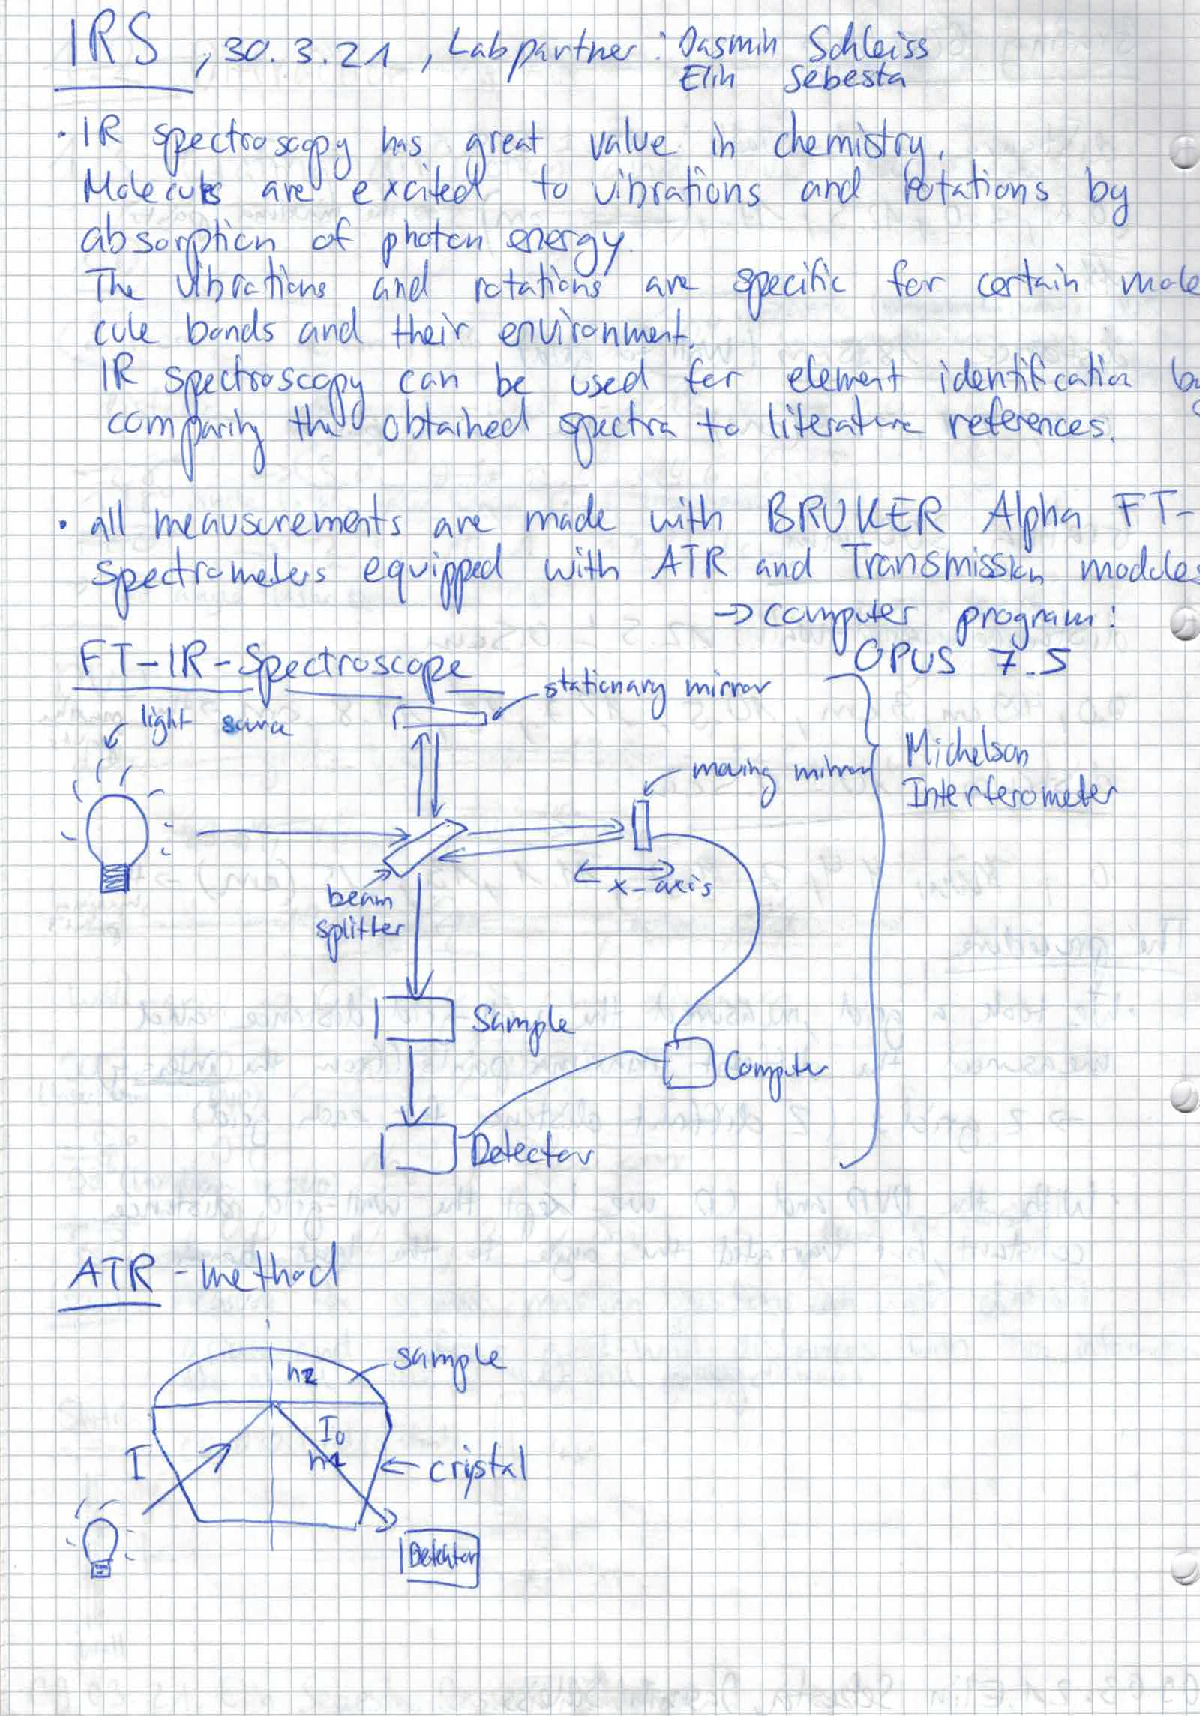
\includegraphics[page=1,width=\textwidth]{LJ.pdf}

\includegraphics[page=2,width=\textwidth]{LJ.pdf}

\includegraphics[page=3,width=\textwidth]{LJ.pdf}

\includegraphics[page=4,width=\textwidth]{LJ.pdf}

\subsection*{A3 - Task sheet}
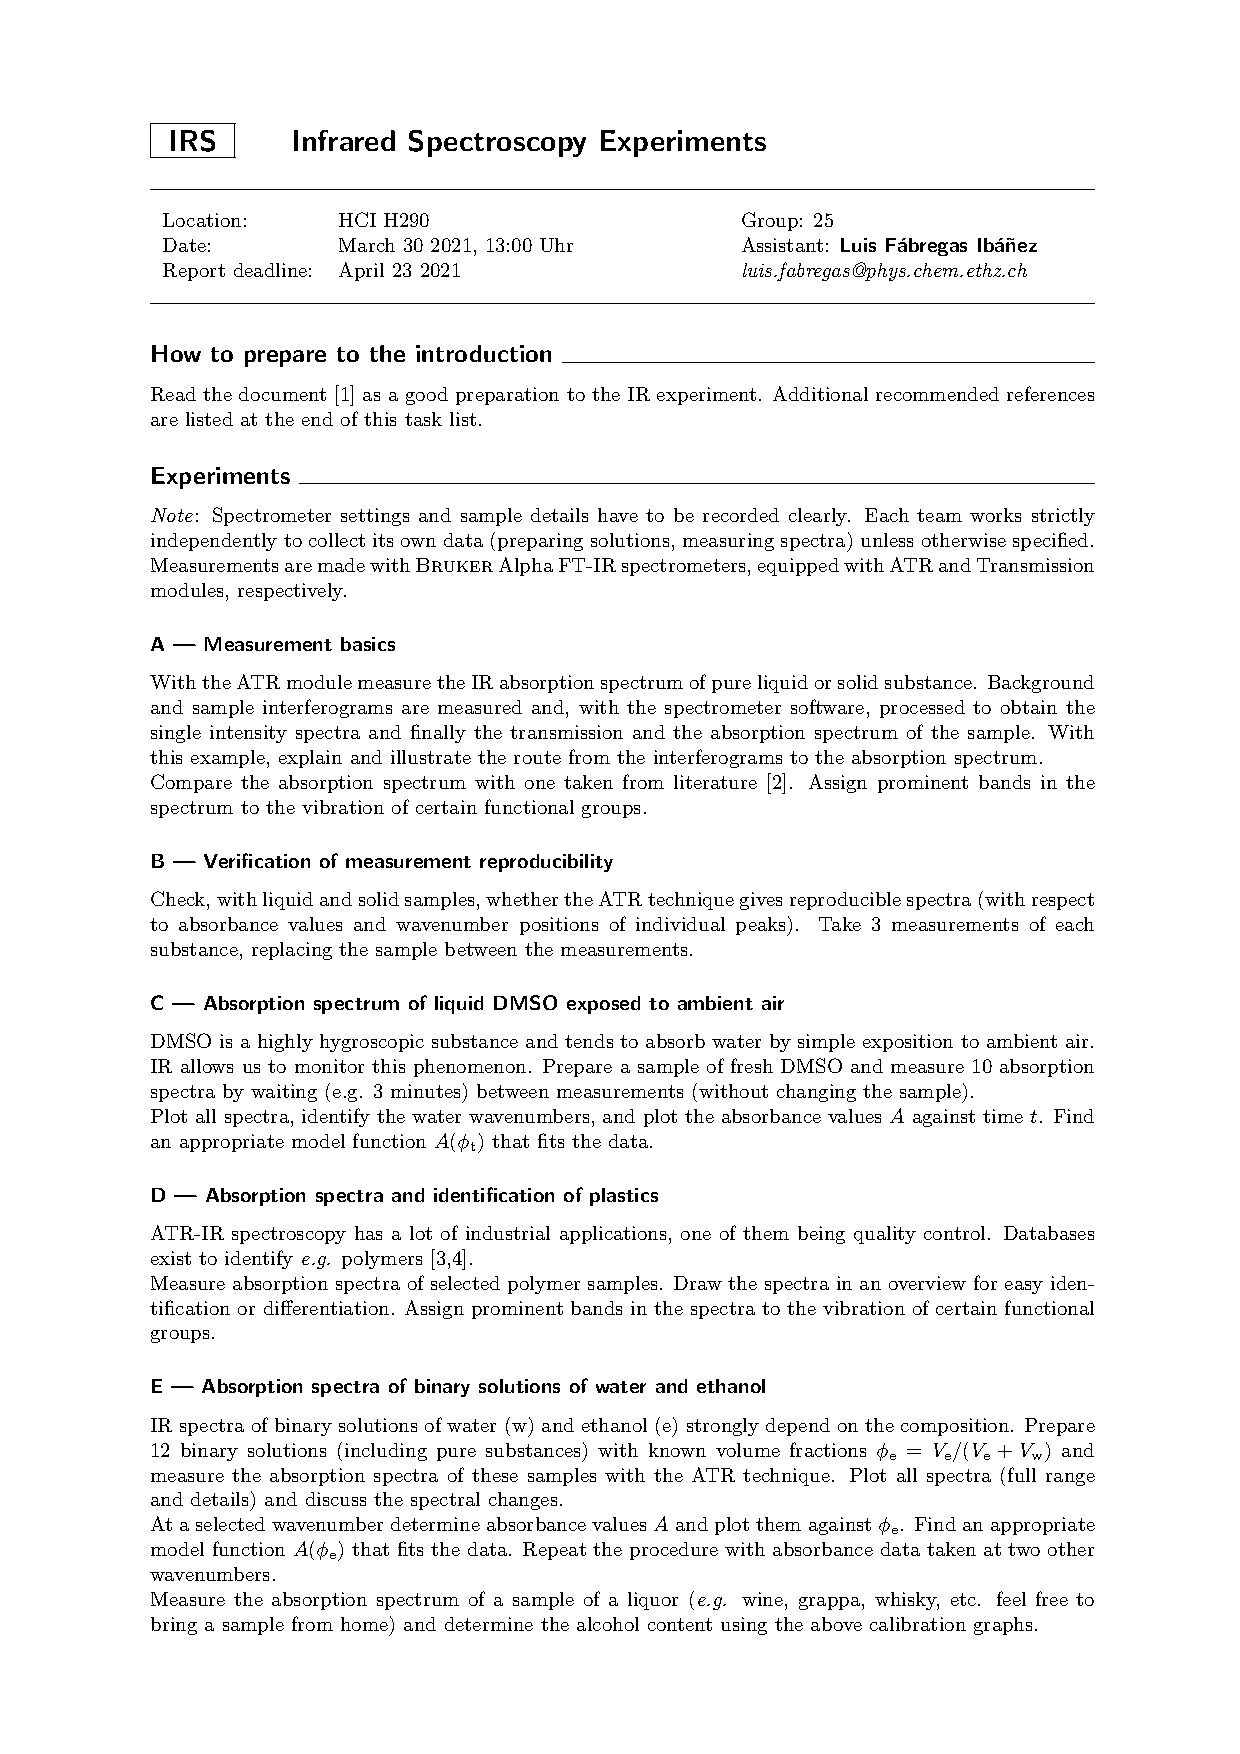
\includegraphics[page = 1,width=\textwidth]{Task.pdf}

\includegraphics[page = 2,width=\textwidth]{Task.pdf}

\subsection*{A4 - Regression summaries}
\subsubsection*{for part C}
The standard errors for the fourth degree polynomial function:

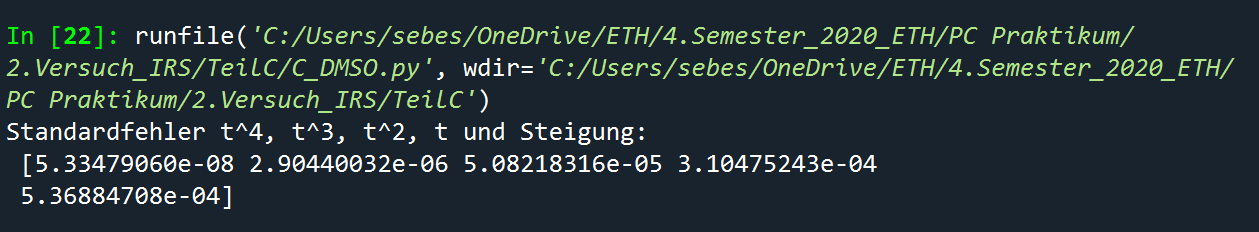
\includegraphics[width=\textwidth]{StandardfehlerC.PNG}
\subsubsection*{for part E}
The standard errors for the three linear regressions:

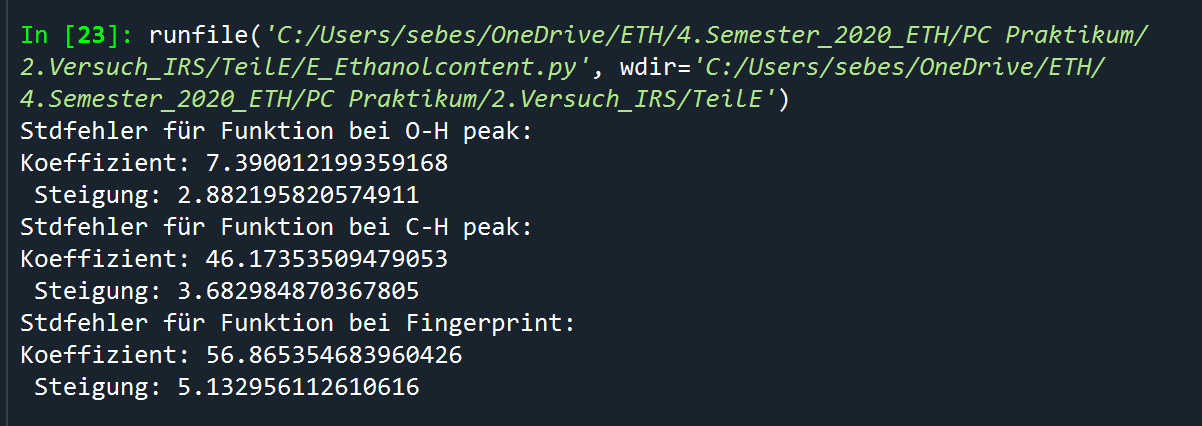
\includegraphics[width=\textwidth]{StandardfehlerE.PNG}

\subsubsection*{for part G}
The regression summary(OLS function used):

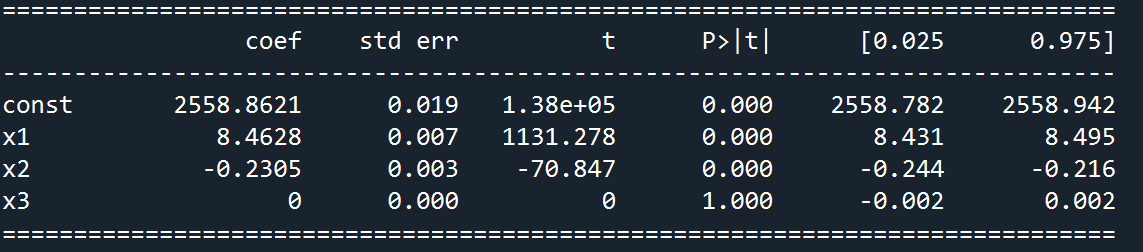
\includegraphics[width=\textwidth]{StandardfehlerG.PNG}

\end{document}





















